\documentclass[twoside]{book}

% Packages required by doxygen
\usepackage{fixltx2e}
\usepackage{calc}
\usepackage{doxygen}
\usepackage[export]{adjustbox} % also loads graphicx
\usepackage{graphicx}
\usepackage[utf8]{inputenc}
\usepackage{makeidx}
\usepackage{multicol}
\usepackage{multirow}
\PassOptionsToPackage{warn}{textcomp}
\usepackage{textcomp}
\usepackage[nointegrals]{wasysym}
\usepackage[table]{xcolor}

% Font selection
\usepackage[T1]{fontenc}
\usepackage[scaled=.90]{helvet}
\usepackage{courier}
\usepackage{amssymb}
\usepackage{sectsty}
\renewcommand{\familydefault}{\sfdefault}
\allsectionsfont{%
  \fontseries{bc}\selectfont%
  \color{darkgray}%
}
\renewcommand{\DoxyLabelFont}{%
  \fontseries{bc}\selectfont%
  \color{darkgray}%
}
\newcommand{\+}{\discretionary{\mbox{\scriptsize$\hookleftarrow$}}{}{}}

% Page & text layout
\usepackage{geometry}
\geometry{%
  a4paper,%
  top=2.5cm,%
  bottom=2.5cm,%
  left=2.5cm,%
  right=2.5cm%
}
\tolerance=750
\hfuzz=15pt
\hbadness=750
\setlength{\emergencystretch}{15pt}
\setlength{\parindent}{0cm}
\setlength{\parskip}{3ex plus 2ex minus 2ex}
\makeatletter
\renewcommand{\paragraph}{%
  \@startsection{paragraph}{4}{0ex}{-1.0ex}{1.0ex}{%
    \normalfont\normalsize\bfseries\SS@parafont%
  }%
}
\renewcommand{\subparagraph}{%
  \@startsection{subparagraph}{5}{0ex}{-1.0ex}{1.0ex}{%
    \normalfont\normalsize\bfseries\SS@subparafont%
  }%
}
\makeatother

% Headers & footers
\usepackage{fancyhdr}
\pagestyle{fancyplain}
\fancyhead[LE]{\fancyplain{}{\bfseries\thepage}}
\fancyhead[CE]{\fancyplain{}{}}
\fancyhead[RE]{\fancyplain{}{\bfseries\leftmark}}
\fancyhead[LO]{\fancyplain{}{\bfseries\rightmark}}
\fancyhead[CO]{\fancyplain{}{}}
\fancyhead[RO]{\fancyplain{}{\bfseries\thepage}}
\fancyfoot[LE]{\fancyplain{}{}}
\fancyfoot[CE]{\fancyplain{}{}}
\fancyfoot[RE]{\fancyplain{}{\bfseries\scriptsize Generated by Doxygen }}
\fancyfoot[LO]{\fancyplain{}{\bfseries\scriptsize Generated by Doxygen }}
\fancyfoot[CO]{\fancyplain{}{}}
\fancyfoot[RO]{\fancyplain{}{}}
\renewcommand{\footrulewidth}{0.4pt}
\renewcommand{\chaptermark}[1]{%
  \markboth{#1}{}%
}
\renewcommand{\sectionmark}[1]{%
  \markright{\thesection\ #1}%
}

% Indices & bibliography
\usepackage{natbib}
\usepackage[titles]{tocloft}
\setcounter{tocdepth}{3}
\setcounter{secnumdepth}{5}
\makeindex

% Custom commands
\newcommand{\clearemptydoublepage}{%
  \newpage{\pagestyle{empty}\cleardoublepage}%
}

\usepackage{caption}
\captionsetup{labelsep=space,justification=centering,font={bf},singlelinecheck=off,skip=4pt,position=top}

%===== C O N T E N T S =====

\begin{document}

% Titlepage & ToC
\pagenumbering{alph}
\begin{titlepage}
\vspace*{7cm}
\begin{center}%
{\Large H\+W4\+\_\+klin2\+\_\+cdbruneau }\\
\vspace*{1cm}
{\large Generated by Doxygen 1.8.13}\\
\end{center}
\end{titlepage}
\clearemptydoublepage
\pagenumbering{roman}
\tableofcontents
\clearemptydoublepage
\pagenumbering{arabic}

%--- Begin generated contents ---
\chapter{Hierarchical Index}
\section{Class Hierarchy}
This inheritance list is sorted roughly, but not completely, alphabetically\+:\begin{DoxyCompactList}
\item \contentsline{section}{Cell}{\pageref{classCell}}{}
\item \contentsline{section}{Grid}{\pageref{classGrid}}{}
\item \contentsline{section}{Organism}{\pageref{classOrganism}}{}
\begin{DoxyCompactList}
\item \contentsline{section}{Ant}{\pageref{classAnt}}{}
\item \contentsline{section}{Doodlebug}{\pageref{classDoodlebug}}{}
\end{DoxyCompactList}
\item \contentsline{section}{Production}{\pageref{classProduction}}{}
\item \contentsline{section}{Tests2}{\pageref{classTests2}}{}
\end{DoxyCompactList}

\chapter{Data Structure Index}
\section{Data Structures}
Here are the data structures with brief descriptions\+:\begin{DoxyCompactList}
\item\contentsline{section}{\textbf{ Ant} }{\pageref{classAnt}}{}
\item\contentsline{section}{\textbf{ Cell} }{\pageref{classCell}}{}
\item\contentsline{section}{\textbf{ Doodlebug} }{\pageref{classDoodlebug}}{}
\item\contentsline{section}{\textbf{ Grid} }{\pageref{classGrid}}{}
\item\contentsline{section}{\textbf{ Organism} }{\pageref{classOrganism}}{}
\item\contentsline{section}{\textbf{ Production} }{\pageref{classProduction}}{}
\item\contentsline{section}{\textbf{ Tests2} }{\pageref{classTests2}}{}
\end{DoxyCompactList}

\chapter{File Index}
\section{File List}
Here is a list of all files with brief descriptions\+:\begin{DoxyCompactList}
\item\contentsline{section}{\textbf{ Ant.\+cpp} }{\pageref{Ant_8cpp}}{}
\item\contentsline{section}{\textbf{ Ant.\+h} }{\pageref{Ant_8h}}{}
\item\contentsline{section}{\textbf{ Ants\+And\+Doodles.\+cpp} }{\pageref{AntsAndDoodles_8cpp}}{}
\item\contentsline{section}{\textbf{ Cell.\+cpp} }{\pageref{Cell_8cpp}}{}
\item\contentsline{section}{\textbf{ Cell.\+h} }{\pageref{Cell_8h}}{}
\item\contentsline{section}{\textbf{ Doodlebug.\+cpp} }{\pageref{Doodlebug_8cpp}}{}
\item\contentsline{section}{\textbf{ Doodlebug.\+h} }{\pageref{Doodlebug_8h}}{}
\item\contentsline{section}{\textbf{ Grid.\+cpp} }{\pageref{Grid_8cpp}}{}
\item\contentsline{section}{\textbf{ Grid.\+h} }{\pageref{Grid_8h}}{}
\item\contentsline{section}{\textbf{ Organism.\+cpp} }{\pageref{Organism_8cpp}}{}
\item\contentsline{section}{\textbf{ Organism.\+h} }{\pageref{Organism_8h}}{}
\item\contentsline{section}{\textbf{ Production.\+cpp} }{\pageref{Production_8cpp}}{}
\item\contentsline{section}{\textbf{ Production.\+h} }{\pageref{Production_8h}}{}
\item\contentsline{section}{\textbf{ Tests2.\+cpp} }{\pageref{Tests2_8cpp}}{}
\item\contentsline{section}{\textbf{ Tests2.\+h} }{\pageref{Tests2_8h}}{}
\end{DoxyCompactList}

\chapter{Data Structure Documentation}
\section{Ant Class Reference}
\label{classAnt}\index{Ant@{Ant}}


{\ttfamily \#include $<$Ant.\+h$>$}

Inheritance diagram for Ant\+:\begin{figure}[H]
\begin{center}
\leavevmode
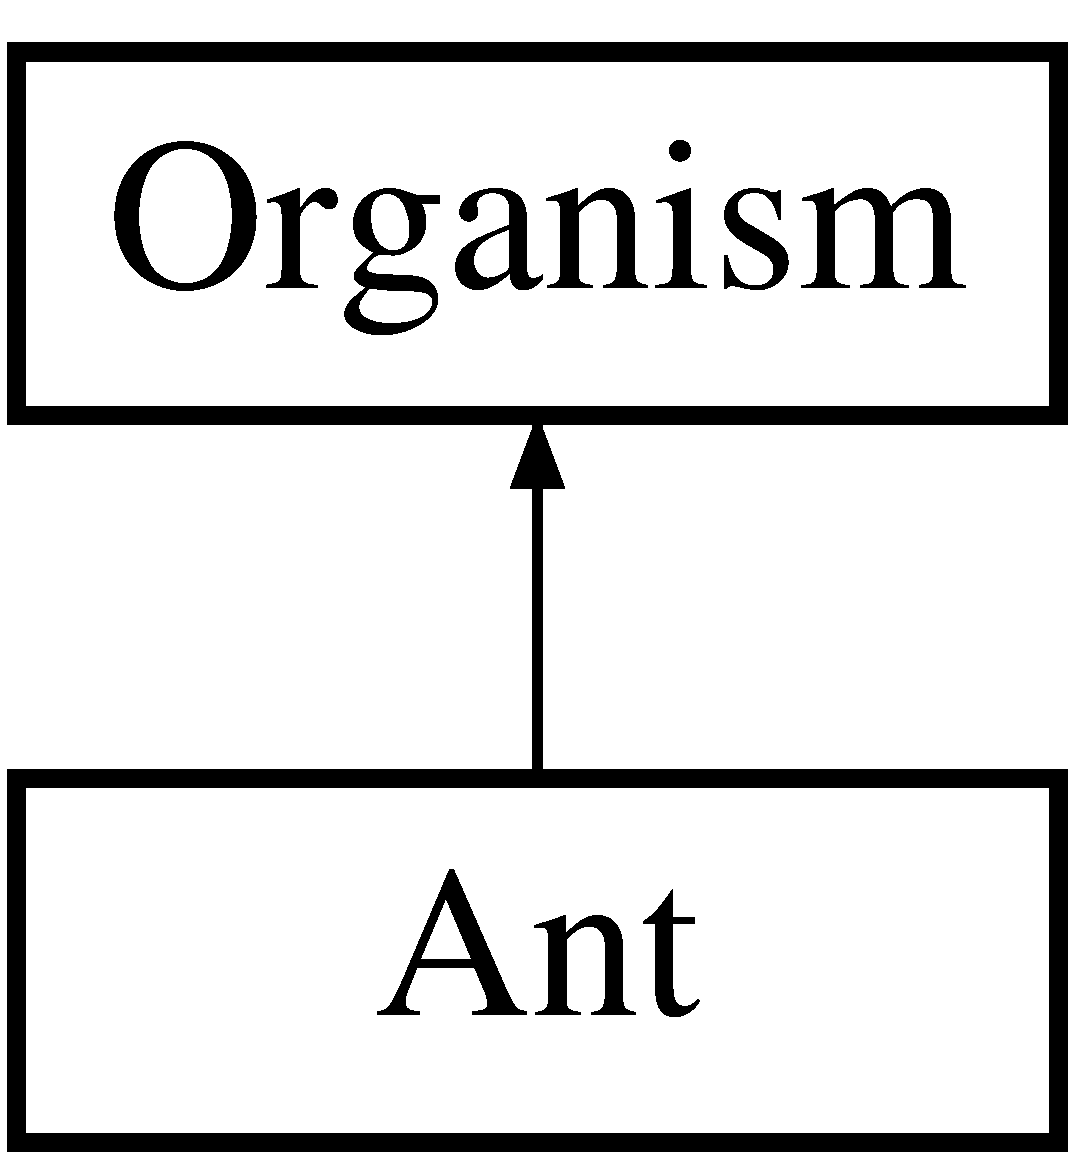
\includegraphics[height=2.000000cm]{classAnt}
\end{center}
\end{figure}
\subsection*{Public Member Functions}
\begin{DoxyCompactItemize}
\item 
\textbf{ Ant} ()
\item 
\textbf{ Ant} (int r=0, int c=0)
\item 
bool \textbf{ breed} (\textbf{ Grid} $\ast$current)
\item 
\textbf{ $\sim$\+Ant} ()
\end{DoxyCompactItemize}
\subsection*{Additional Inherited Members}


\subsection{Constructor \& Destructor Documentation}
\mbox{\label{classAnt_ad6c1a8f70419877f7a3e2c9c557f913d}} 
\index{Ant@{Ant}!Ant@{Ant}}
\index{Ant@{Ant}!Ant@{Ant}}
\subsubsection{Ant()\hspace{0.1cm}{\footnotesize\ttfamily [1/2]}}
{\footnotesize\ttfamily Ant\+::\+Ant (\begin{DoxyParamCaption}{ }\end{DoxyParamCaption})}

Function is the default constructor for an \doxyref{Ant}{p.}{classAnt} object that instantiates an \doxyref{Ant}{p.}{classAnt} object. \mbox{\label{classAnt_afcb9b285a5aa4b329e7eb5783970d85f}} 
\index{Ant@{Ant}!Ant@{Ant}}
\index{Ant@{Ant}!Ant@{Ant}}
\subsubsection{Ant()\hspace{0.1cm}{\footnotesize\ttfamily [2/2]}}
{\footnotesize\ttfamily Ant\+::\+Ant (\begin{DoxyParamCaption}\item[{int}]{r = {\ttfamily 0},  }\item[{int}]{c = {\ttfamily 0} }\end{DoxyParamCaption})}

Function is another constructor for an \doxyref{Ant}{p.}{classAnt} object that instantiates an \doxyref{Ant}{p.}{classAnt} object and sets the rows to the given parameter r, and sets the columns to the given parameter c.


\begin{DoxyParams}{Parameters}
{\em r} & The row that the ant will be instantiated on. \\
\hline
{\em c} & The column that the ant will be instantiated on. \\
\hline
\end{DoxyParams}


References Organism\+::col, and Organism\+::row.

\mbox{\label{classAnt_a33ca6bd592236726a18a2159908e4116}} 
\index{Ant@{Ant}!````~Ant@{$\sim$\+Ant}}
\index{````~Ant@{$\sim$\+Ant}!Ant@{Ant}}
\subsubsection{$\sim$\+Ant()}
{\footnotesize\ttfamily Ant\+::$\sim$\+Ant (\begin{DoxyParamCaption}{ }\end{DoxyParamCaption})}

Function is a destructor that takes the \doxyref{Ant}{p.}{classAnt} object and deletes it once the program is done using the object. 

\subsection{Member Function Documentation}
\mbox{\label{classAnt_ab51f7167f7e9b8e942a1ca5cbcecc3ba}} 
\index{Ant@{Ant}!breed@{breed}}
\index{breed@{breed}!Ant@{Ant}}
\subsubsection{breed()}
{\footnotesize\ttfamily bool Ant\+::breed (\begin{DoxyParamCaption}\item[{\textbf{ Grid} $\ast$}]{current }\end{DoxyParamCaption})\hspace{0.3cm}{\ttfamily [virtual]}}

Function tells whether if an ant will breed or not.


\begin{DoxyParams}{Parameters}
{\em current} & A pointer to the current board that the game is being played on. \\
\hline
\end{DoxyParams}
\begin{DoxyReturn}{Returns}
status A boolean value that indicates true if an ant can breed and false if the ant cannot breed. 
\end{DoxyReturn}


Implements \textbf{ Organism} \doxyref{}{p.}{classOrganism_aeecced266ac9dd055a0a0caf57379fb7}.



References Organism\+::col, Grid\+::create\+Organism(), Grid\+::find\+Move(), Organism\+::row, and Organism\+::step\+Count.



Referenced by Tests2\+::ants\+Breed\+Test().



The documentation for this class was generated from the following files\+:\begin{DoxyCompactItemize}
\item 
\textbf{ Ant.\+h}\item 
\textbf{ Ant.\+cpp}\end{DoxyCompactItemize}

\section{Cell Class Reference}
\label{classCell}\index{Cell@{Cell}}


{\ttfamily \#include $<$Cell.\+h$>$}

\subsection*{Public Member Functions}
\begin{DoxyCompactItemize}
\item 
\textbf{ Cell} ()
\item 
bool \textbf{ set\+Occupant} (\textbf{ occupation\+Status} g)
\item 
\textbf{ occupation\+Status} \textbf{ get\+Occupant} ()
\item 
void \textbf{ print\+Cell} ()
\item 
\textbf{ Organism} $\ast$ \textbf{ get\+Current\+Organism} ()
\item 
\textbf{ Organism} $\ast$ \textbf{ set\+Current\+Organism} (\textbf{ Organism} $\ast$new\+Occupant)
\item 
virtual \textbf{ $\sim$\+Cell} ()
\end{DoxyCompactItemize}
\subsection*{Private Attributes}
\begin{DoxyCompactItemize}
\item 
\textbf{ Organism} $\ast$ \textbf{ occupant}
\item 
\textbf{ occupation\+Status} \textbf{ guest} = \textbf{ empty}
\end{DoxyCompactItemize}


\subsection{Constructor \& Destructor Documentation}
\mbox{\label{classCell_a394510643e8664cf12b5efaf5cb99f71}} 
\index{Cell@{Cell}!Cell@{Cell}}
\index{Cell@{Cell}!Cell@{Cell}}
\subsubsection{Cell()}
{\footnotesize\ttfamily Cell\+::\+Cell (\begin{DoxyParamCaption}{ }\end{DoxyParamCaption})}

Function is the default constructor for a \doxyref{Cell}{p.}{classCell} object that instantiates a \doxyref{Cell}{p.}{classCell} object with an empty guest. 

References empty, guest, and occupant.

\mbox{\label{classCell_a9fa559f7a28e2b4336c6879ca09304d8}} 
\index{Cell@{Cell}!````~Cell@{$\sim$\+Cell}}
\index{````~Cell@{$\sim$\+Cell}!Cell@{Cell}}
\subsubsection{$\sim$\+Cell()}
{\footnotesize\ttfamily Cell\+::$\sim$\+Cell (\begin{DoxyParamCaption}{ }\end{DoxyParamCaption})\hspace{0.3cm}{\ttfamily [virtual]}}

Function is a destructor that takes the \doxyref{Cell}{p.}{classCell} object and deletes it once the program is done using the object. 

Referenced by Grid\+::$\sim$\+Grid().



\subsection{Member Function Documentation}
\mbox{\label{classCell_a345a66766f6af82f932f2bfc2510ba51}} 
\index{Cell@{Cell}!get\+Current\+Organism@{get\+Current\+Organism}}
\index{get\+Current\+Organism@{get\+Current\+Organism}!Cell@{Cell}}
\subsubsection{get\+Current\+Organism()}
{\footnotesize\ttfamily \textbf{ Organism} $\ast$ Cell\+::get\+Current\+Organism (\begin{DoxyParamCaption}{ }\end{DoxyParamCaption})}

Function that returns the \doxyref{Cell}{p.}{classCell}\textquotesingle{}s occupant.

\begin{DoxyReturn}{Returns}
occupant The current occupant of a cell. 
\end{DoxyReturn}


References occupant.



Referenced by Grid\+::delete\+Organism(), Grid\+::get\+Cell\+Organism(), and Grid\+::move\+Organism().

\mbox{\label{classCell_a7dcb8bc75a2e2591b3fd52b5f7c28ab1}} 
\index{Cell@{Cell}!get\+Occupant@{get\+Occupant}}
\index{get\+Occupant@{get\+Occupant}!Cell@{Cell}}
\subsubsection{get\+Occupant()}
{\footnotesize\ttfamily \textbf{ occupation\+Status} Cell\+::get\+Occupant (\begin{DoxyParamCaption}{ }\end{DoxyParamCaption})}

Function that returns the \doxyref{Cell}{p.}{classCell}\textquotesingle{}s occupancy status.

\begin{DoxyReturn}{Returns}
guest A value that indicates the occupancy status of a cell. 
\end{DoxyReturn}


References guest.



Referenced by Grid\+::get\+Cell\+Occupant().

\mbox{\label{classCell_a930a4ccf1ee9f6168c6b72bb0c3a5e8d}} 
\index{Cell@{Cell}!print\+Cell@{print\+Cell}}
\index{print\+Cell@{print\+Cell}!Cell@{Cell}}
\subsubsection{print\+Cell()}
{\footnotesize\ttfamily void Cell\+::print\+Cell (\begin{DoxyParamCaption}{ }\end{DoxyParamCaption})}

Function that prints a character representing the current occupation status of the cell. If the occupation status is ant, this function prints \textquotesingle{}o\textquotesingle{} If the occupation status is a doodlebug, this function prints \textquotesingle{}x\textquotesingle{} If the occupation status is empty, this function prints \textquotesingle{} \textquotesingle{} 

References ant, doodlebug, empty, and guest.



Referenced by Grid\+::print\+Grid(), and Tests2\+::print\+Grid\+And\+Cell\+Test().

\mbox{\label{classCell_a8e9e7c2dcb9f20238931da684451a9f4}} 
\index{Cell@{Cell}!set\+Current\+Organism@{set\+Current\+Organism}}
\index{set\+Current\+Organism@{set\+Current\+Organism}!Cell@{Cell}}
\subsubsection{set\+Current\+Organism()}
{\footnotesize\ttfamily \textbf{ Organism} $\ast$ Cell\+::set\+Current\+Organism (\begin{DoxyParamCaption}\item[{\textbf{ Organism} $\ast$}]{new\+Occupant }\end{DoxyParamCaption})}

Function that sets the \doxyref{Cell}{p.}{classCell}\textquotesingle{}s occupant.


\begin{DoxyParams}{Parameters}
{\em new\+Occupant} & A pointer to an organism object that the cell\textquotesingle{}s organism will be set to. \\
\hline
\end{DoxyParams}
\begin{DoxyReturn}{Returns}
occupant The new occupant of a cell. 
\end{DoxyReturn}


References occupant.



Referenced by Grid\+::create\+Organism(), Grid\+::delete\+Organism(), Grid\+::move\+Organism(), and Grid\+::set\+Cell\+Organism().

\mbox{\label{classCell_a2346933316b45d87264d50e563c2f895}} 
\index{Cell@{Cell}!set\+Occupant@{set\+Occupant}}
\index{set\+Occupant@{set\+Occupant}!Cell@{Cell}}
\subsubsection{set\+Occupant()}
{\footnotesize\ttfamily bool Cell\+::set\+Occupant (\begin{DoxyParamCaption}\item[{\textbf{ occupation\+Status}}]{g }\end{DoxyParamCaption})}

Function is a constructor for a cell object that instantiates a cell object and sets the occupancy status to the passed in parameter, g, and returns the result. \begin{DoxyReturn}{Returns}
result A boolean value that indicates true if the occupant status has been set and false if the status has not been set because the \doxyref{Cell}{p.}{classCell} was occupied. 
\end{DoxyReturn}


References empty, and guest.



Referenced by Grid\+::create\+Organism(), Grid\+::delete\+Organism(), and Grid\+::set\+Cell\+Occupant().



\subsection{Field Documentation}
\mbox{\label{classCell_aafc273a5125cf29742a8df6f5a5a881c}} 
\index{Cell@{Cell}!guest@{guest}}
\index{guest@{guest}!Cell@{Cell}}
\subsubsection{guest}
{\footnotesize\ttfamily \textbf{ occupation\+Status} Cell\+::guest = \textbf{ empty}\hspace{0.3cm}{\ttfamily [private]}}



Referenced by Cell(), get\+Occupant(), print\+Cell(), and set\+Occupant().

\mbox{\label{classCell_a40b81375938f1f13342c34dc1ac692b2}} 
\index{Cell@{Cell}!occupant@{occupant}}
\index{occupant@{occupant}!Cell@{Cell}}
\subsubsection{occupant}
{\footnotesize\ttfamily \textbf{ Organism}$\ast$ Cell\+::occupant\hspace{0.3cm}{\ttfamily [private]}}



Referenced by Cell(), get\+Current\+Organism(), and set\+Current\+Organism().



The documentation for this class was generated from the following files\+:\begin{DoxyCompactItemize}
\item 
\textbf{ Cell.\+h}\item 
\textbf{ Cell.\+cpp}\end{DoxyCompactItemize}

\section{Doodlebug Class Reference}
\label{classDoodlebug}\index{Doodlebug@{Doodlebug}}


{\ttfamily \#include $<$Doodlebug.\+h$>$}

Inheritance diagram for Doodlebug\+:\begin{figure}[H]
\begin{center}
\leavevmode
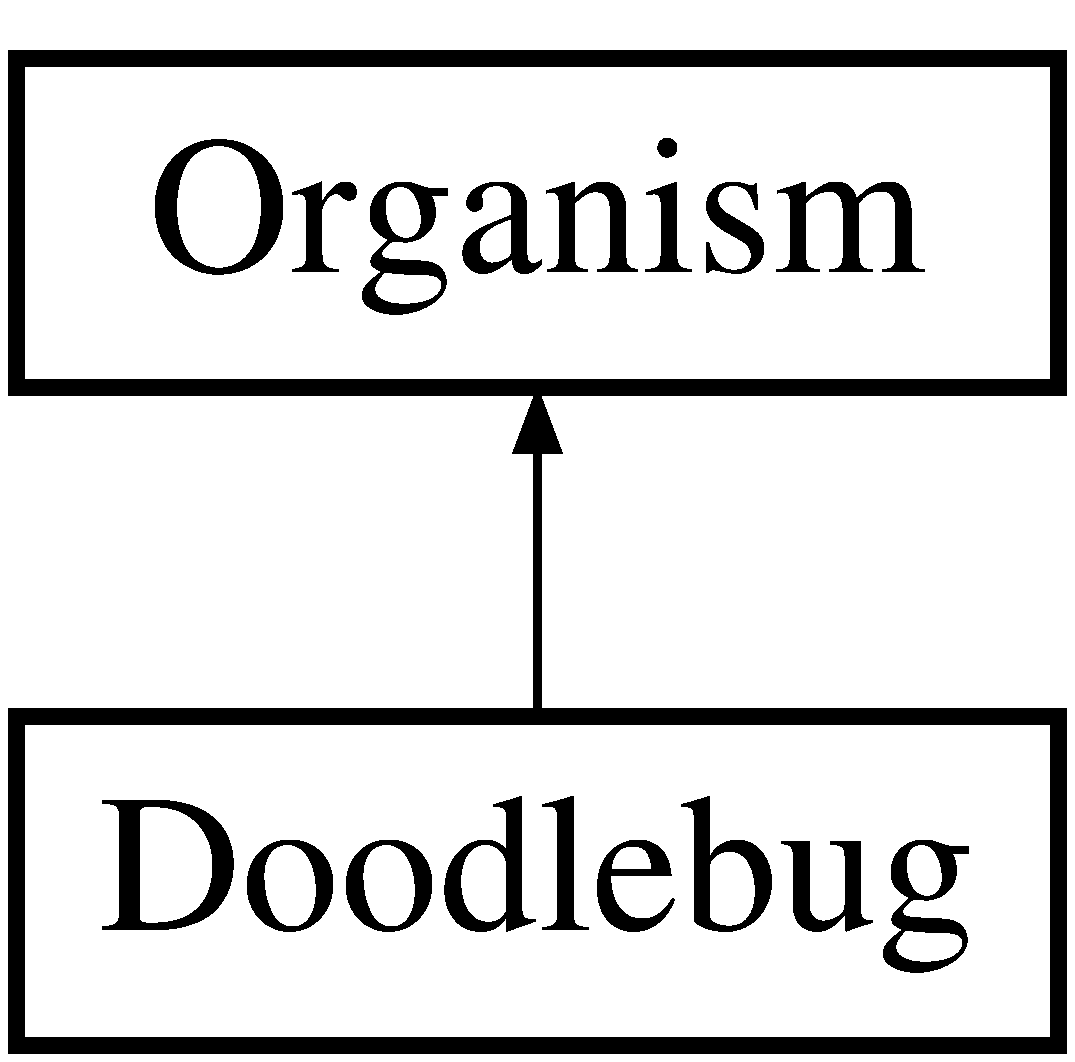
\includegraphics[height=2.000000cm]{classDoodlebug}
\end{center}
\end{figure}
\subsection*{Public Member Functions}
\begin{DoxyCompactItemize}
\item 
\textbf{ Doodlebug} (int r, int c)
\item 
int \textbf{ get\+Starve\+Count} ()
\item 
void \textbf{ set\+Starve\+Count} (int count)
\item 
bool \textbf{ move} (\textbf{ Grid} $\ast$current)
\item 
bool \textbf{ breed} (\textbf{ Grid} $\ast$current)
\item 
bool \textbf{ eat} (\textbf{ Grid} $\ast$current)
\item 
bool \textbf{ starve} ()
\item 
virtual \textbf{ $\sim$\+Doodlebug} ()
\end{DoxyCompactItemize}
\subsection*{Private Attributes}
\begin{DoxyCompactItemize}
\item 
int \textbf{ starve\+Count} = 0
\end{DoxyCompactItemize}
\subsection*{Additional Inherited Members}


\subsection{Constructor \& Destructor Documentation}
\mbox{\label{classDoodlebug_a0009927ec98eb6203900af3637fb3e3a}} 
\index{Doodlebug@{Doodlebug}!Doodlebug@{Doodlebug}}
\index{Doodlebug@{Doodlebug}!Doodlebug@{Doodlebug}}
\subsubsection{Doodlebug()}
{\footnotesize\ttfamily Doodlebug\+::\+Doodlebug (\begin{DoxyParamCaption}\item[{int}]{r,  }\item[{int}]{c }\end{DoxyParamCaption})}

Function is the default constructor for a \doxyref{Doodlebug}{p.}{classDoodlebug} object that instantiates a \doxyref{Doodlebug}{p.}{classDoodlebug} object.


\begin{DoxyParams}{Parameters}
{\em r} & The row that the doodlebug will be instantiated on. \\
\hline
{\em c} & The column that the doodlebug will be instantiated on. \\
\hline
\end{DoxyParams}


References Organism\+::col, and Organism\+::row.

\mbox{\label{classDoodlebug_ac318cc9acbd9a3af52348a236070d891}} 
\index{Doodlebug@{Doodlebug}!````~Doodlebug@{$\sim$\+Doodlebug}}
\index{````~Doodlebug@{$\sim$\+Doodlebug}!Doodlebug@{Doodlebug}}
\subsubsection{$\sim$\+Doodlebug()}
{\footnotesize\ttfamily Doodlebug\+::$\sim$\+Doodlebug (\begin{DoxyParamCaption}{ }\end{DoxyParamCaption})\hspace{0.3cm}{\ttfamily [virtual]}}

Function is a destructor that takes the \doxyref{Doodlebug}{p.}{classDoodlebug} object and deletes it once the program is done using the object. 

\subsection{Member Function Documentation}
\mbox{\label{classDoodlebug_a6aa05cce6d3d7df55d9c3787c01fd9b2}} 
\index{Doodlebug@{Doodlebug}!breed@{breed}}
\index{breed@{breed}!Doodlebug@{Doodlebug}}
\subsubsection{breed()}
{\footnotesize\ttfamily bool Doodlebug\+::breed (\begin{DoxyParamCaption}\item[{\textbf{ Grid} $\ast$}]{current }\end{DoxyParamCaption})\hspace{0.3cm}{\ttfamily [virtual]}}

Functions tells whether if the doodlebug can breed or not.


\begin{DoxyParams}{Parameters}
{\em current} & A pointer to the current board that the game is being played on. \\
\hline
\end{DoxyParams}
\begin{DoxyReturn}{Returns}
status A boolean value that indicates true if a doodlebug can breed and false if the doodlebug cannot breed. 
\end{DoxyReturn}


Implements \textbf{ Organism} \doxyref{}{p.}{classOrganism_aeecced266ac9dd055a0a0caf57379fb7}.



References Organism\+::col, Grid\+::create\+Organism(), Grid\+::find\+Move(), Organism\+::row, and Organism\+::step\+Count.



Referenced by Tests2\+::doodle\+Breed\+Test().

\mbox{\label{classDoodlebug_a00a3a3e9a9b82d6dc9affae5c4e01630}} 
\index{Doodlebug@{Doodlebug}!eat@{eat}}
\index{eat@{eat}!Doodlebug@{Doodlebug}}
\subsubsection{eat()}
{\footnotesize\ttfamily bool Doodlebug\+::eat (\begin{DoxyParamCaption}\item[{\textbf{ Grid} $\ast$}]{current }\end{DoxyParamCaption})\hspace{0.3cm}{\ttfamily [virtual]}}

Functions tells whether if the doodlebug can eat or not.


\begin{DoxyParams}{Parameters}
{\em current} & A pointer to the current board that the game is being played on. \\
\hline
\end{DoxyParams}
\begin{DoxyReturn}{Returns}
status A boolean value that indicates true if a doodlebug can eat and false if the doodlebug cannot eat. 
\end{DoxyReturn}


Reimplemented from \textbf{ Organism} \doxyref{}{p.}{classOrganism_a8305e732b48c3a16dbc83b8a42eaa52a}.



References Organism\+::col, Grid\+::delete\+Organism(), Grid\+::find\+Food(), Grid\+::move\+Organism(), and Organism\+::row.



Referenced by Tests2\+::ants\+Die\+Test(), Tests2\+::doodle\+Eat\+Test(), and move().

\mbox{\label{classDoodlebug_a936c2ef9653914f6aecef20a2abe4097}} 
\index{Doodlebug@{Doodlebug}!get\+Starve\+Count@{get\+Starve\+Count}}
\index{get\+Starve\+Count@{get\+Starve\+Count}!Doodlebug@{Doodlebug}}
\subsubsection{get\+Starve\+Count()}
{\footnotesize\ttfamily int Doodlebug\+::get\+Starve\+Count (\begin{DoxyParamCaption}{ }\end{DoxyParamCaption})}

Returns the \doxyref{Organism}{p.}{classOrganism}\textquotesingle{}s current starve\+Count; 

References starve\+Count.

\mbox{\label{classDoodlebug_ae411913efc4e52c0f726c537dacbb778}} 
\index{Doodlebug@{Doodlebug}!move@{move}}
\index{move@{move}!Doodlebug@{Doodlebug}}
\subsubsection{move()}
{\footnotesize\ttfamily bool Doodlebug\+::move (\begin{DoxyParamCaption}\item[{\textbf{ Grid} $\ast$}]{current }\end{DoxyParamCaption})\hspace{0.3cm}{\ttfamily [virtual]}}

Functions tells whether if the doodlebug will move or not.


\begin{DoxyParams}{Parameters}
{\em current} & A pointer to the current board that the game is being played on. \\
\hline
\end{DoxyParams}
\begin{DoxyReturn}{Returns}
status A boolean value that indicates true if a doodlebug can move and false if the doodlebug cannot move. 
\end{DoxyReturn}


Reimplemented from \textbf{ Organism} \doxyref{}{p.}{classOrganism_ad83535a041d8cc6543a8f68c80c14122}.



References eat(), Organism\+::move(), and starve\+Count.



Referenced by Tests2\+::doodle\+Move\+Test().

\mbox{\label{classDoodlebug_aa4981f015adc040ad5c0ff3b9931e4fa}} 
\index{Doodlebug@{Doodlebug}!set\+Starve\+Count@{set\+Starve\+Count}}
\index{set\+Starve\+Count@{set\+Starve\+Count}!Doodlebug@{Doodlebug}}
\subsubsection{set\+Starve\+Count()}
{\footnotesize\ttfamily void Doodlebug\+::set\+Starve\+Count (\begin{DoxyParamCaption}\item[{int}]{count }\end{DoxyParamCaption})}

Sets the \doxyref{Organism}{p.}{classOrganism}\textquotesingle{}s starve\+Count to the passed in parameter count;


\begin{DoxyParams}{Parameters}
{\em count} & The amount of plays that the doodlebug has been starving for. \\
\hline
\end{DoxyParams}


References starve\+Count.

\mbox{\label{classDoodlebug_a7f1c26c8458f3811680c778362c0e374}} 
\index{Doodlebug@{Doodlebug}!starve@{starve}}
\index{starve@{starve}!Doodlebug@{Doodlebug}}
\subsubsection{starve()}
{\footnotesize\ttfamily bool Doodlebug\+::starve (\begin{DoxyParamCaption}{ }\end{DoxyParamCaption})\hspace{0.3cm}{\ttfamily [virtual]}}

Returns whether or not the \doxyref{Doodlebug}{p.}{classDoodlebug} has starved. 

Reimplemented from \textbf{ Organism} \doxyref{}{p.}{classOrganism_ad1456a1f22de197cc74ca8cf5a1a0189}.



References starve\+Count.



\subsection{Field Documentation}
\mbox{\label{classDoodlebug_a18e809db6a20c787bbff7c9fe4d92f52}} 
\index{Doodlebug@{Doodlebug}!starve\+Count@{starve\+Count}}
\index{starve\+Count@{starve\+Count}!Doodlebug@{Doodlebug}}
\subsubsection{starve\+Count}
{\footnotesize\ttfamily int Doodlebug\+::starve\+Count = 0\hspace{0.3cm}{\ttfamily [private]}}



Referenced by get\+Starve\+Count(), move(), set\+Starve\+Count(), and starve().



The documentation for this class was generated from the following files\+:\begin{DoxyCompactItemize}
\item 
\textbf{ Doodlebug.\+h}\item 
\textbf{ Doodlebug.\+cpp}\end{DoxyCompactItemize}

\section{Grid Class Reference}
\label{classGrid}\index{Grid@{Grid}}


{\ttfamily \#include $<$Grid.\+h$>$}

\subsection*{Public Member Functions}
\begin{DoxyCompactItemize}
\item 
\textbf{ Grid} ()
\item 
\textbf{ Grid} (int n\+Squares\+On\+A\+Side)
\item 
bool \textbf{ set\+Cell\+Occupant} (int r, int c, \textbf{ occupation\+Status} g)
\item 
\textbf{ occupation\+Status} \textbf{ get\+Cell\+Occupant} (int r, int c)
\item 
\textbf{ occupation\+Status} $\ast$ \textbf{ check\+Neighbors} (int r, int c)
\item 
bool $\ast$ \textbf{ find\+Food} (int r, int c)
\item 
bool $\ast$ \textbf{ find\+Move} (int r, int c)
\item 
void \textbf{ move\+Organism} (int r\+\_\+old, int c\+\_\+old, int r\+\_\+new, int c\+\_\+new)
\item 
void \textbf{ set\+Cell\+Organism} (int r, int c, \textbf{ Organism} $\ast$g)
\item 
\textbf{ Organism} $\ast$ \textbf{ get\+Cell\+Organism} (int r, int c)
\item 
\textbf{ Cell} \textbf{ get\+Cell} (int r, int c)
\item 
void \textbf{ print\+Grid} ()
\item 
void \textbf{ delete\+Organism} (int r, int c)
\item 
bool \textbf{ create\+Organism} (int r, int c, \textbf{ Organism} $\ast$mother)
\item 
virtual \textbf{ $\sim$\+Grid} ()
\end{DoxyCompactItemize}
\subsection*{Private Attributes}
\begin{DoxyCompactItemize}
\item 
int \textbf{ n} =0
\item 
\textbf{ Cell} $\ast$$\ast$ \textbf{ my\+Grid\+Cells\+\_\+ptr\+\_\+array} = (\textbf{ Cell}$\ast$$\ast$)nullptr
\end{DoxyCompactItemize}


\subsection{Constructor \& Destructor Documentation}
\mbox{\label{classGrid_a4ac9ff4f63552b4c61ff90fcb35ad66c}} 
\index{Grid@{Grid}!Grid@{Grid}}
\index{Grid@{Grid}!Grid@{Grid}}
\subsubsection{Grid()\hspace{0.1cm}{\footnotesize\ttfamily [1/2]}}
{\footnotesize\ttfamily Grid\+::\+Grid (\begin{DoxyParamCaption}{ }\end{DoxyParamCaption})}

Function is the default constructor for a \doxyref{Grid}{p.}{classGrid} object that instantiates a \doxyref{Grid}{p.}{classGrid} object with the default grid value set to 10.. \mbox{\label{classGrid_af35b0accda3471400d55eae5ea07cd40}} 
\index{Grid@{Grid}!Grid@{Grid}}
\index{Grid@{Grid}!Grid@{Grid}}
\subsubsection{Grid()\hspace{0.1cm}{\footnotesize\ttfamily [2/2]}}
{\footnotesize\ttfamily Grid\+::\+Grid (\begin{DoxyParamCaption}\item[{int}]{n\+Squares\+On\+A\+Side }\end{DoxyParamCaption})}

Function is another constructor for a \doxyref{Grid}{p.}{classGrid} object that instantiates a grid object and sets the size of the grid, n, to the given parameter n\+Squares\+On\+Side, and allocates a array of pointers with n amount of row pointers and allocates memory for n amount of columns in each row.


\begin{DoxyParams}{Parameters}
{\em n\+Squares\+On\+A\+Side} & The number of rows and columns on each side of the newly created grid. \\
\hline
\end{DoxyParams}


References my\+Grid\+Cells\+\_\+ptr\+\_\+array, and n.

\mbox{\label{classGrid_a3661d0a7f998caaaf8627d7a67072116}} 
\index{Grid@{Grid}!````~Grid@{$\sim$\+Grid}}
\index{````~Grid@{$\sim$\+Grid}!Grid@{Grid}}
\subsubsection{$\sim$\+Grid()}
{\footnotesize\ttfamily Grid\+::$\sim$\+Grid (\begin{DoxyParamCaption}{ }\end{DoxyParamCaption})\hspace{0.3cm}{\ttfamily [virtual]}}

Function is a destructor that takes the \doxyref{Grid}{p.}{classGrid} object and deletes it once the program is done using the object. 

References my\+Grid\+Cells\+\_\+ptr\+\_\+array, n, and Cell\+::$\sim$\+Cell().



Referenced by Tests2\+::grid\+Test().



\subsection{Member Function Documentation}
\mbox{\label{classGrid_a04a90827b285b2a8d5e2d05ef1a973ad}} 
\index{Grid@{Grid}!check\+Neighbors@{check\+Neighbors}}
\index{check\+Neighbors@{check\+Neighbors}!Grid@{Grid}}
\subsubsection{check\+Neighbors()}
{\footnotesize\ttfamily \textbf{ occupation\+Status} $\ast$ Grid\+::check\+Neighbors (\begin{DoxyParamCaption}\item[{int}]{r,  }\item[{int}]{c }\end{DoxyParamCaption})}

Returns a pointer to an array of occupation statuses that represents the occupied status for the positions North , South, East, West specifically in that order.


\begin{DoxyParams}{Parameters}
{\em r} & The row of the cell whose neighbors we check. \\
\hline
{\em c} & The column of the cell whose neighbors we check. \\
\hline
\end{DoxyParams}
\begin{DoxyReturn}{Returns}
values An array of boolean values that determines if the cells north, south, east, and west are occupied. 
\end{DoxyReturn}


References get\+Cell\+Occupant().



Referenced by Tests2\+::check\+Neighbors\+Test(), find\+Food(), and find\+Move().

\mbox{\label{classGrid_ac5ebe66d2ed90bd76f326047f3b10dbd}} 
\index{Grid@{Grid}!create\+Organism@{create\+Organism}}
\index{create\+Organism@{create\+Organism}!Grid@{Grid}}
\subsubsection{create\+Organism()}
{\footnotesize\ttfamily bool Grid\+::create\+Organism (\begin{DoxyParamCaption}\item[{int}]{r,  }\item[{int}]{c,  }\item[{\textbf{ Organism} $\ast$}]{mother }\end{DoxyParamCaption})}

Function creates a new organism, an ant or a doodlebug depending on the type of the mother organism, in the place of the given row and column.


\begin{DoxyParams}{Parameters}
{\em r} & The row of the cell whose organism is to be deleted. \\
\hline
{\em c} & The column of the cell whose organism is to be deleted. \\
\hline
{\em mother} & The organism of the original cell that the new cell will take after of. \\
\hline
\end{DoxyParams}


References ant, doodlebug, get\+Cell\+Occupant(), Organism\+::is\+Prey(), my\+Grid\+Cells\+\_\+ptr\+\_\+array, Cell\+::set\+Current\+Organism(), Cell\+::set\+Occupant(), and unavailable.



Referenced by Ant\+::breed(), and Doodlebug\+::breed().

\mbox{\label{classGrid_a29a9b20c00c6545aab70a1a667a19a24}} 
\index{Grid@{Grid}!delete\+Organism@{delete\+Organism}}
\index{delete\+Organism@{delete\+Organism}!Grid@{Grid}}
\subsubsection{delete\+Organism()}
{\footnotesize\ttfamily void Grid\+::delete\+Organism (\begin{DoxyParamCaption}\item[{int}]{r,  }\item[{int}]{c }\end{DoxyParamCaption})}

Function deletes the organism in the location of the passed in parameters, r, and c.


\begin{DoxyParams}{Parameters}
{\em r} & The row of the cell whose organism is to be deleted. \\
\hline
{\em c} & The column of the cell whose organism is to be deleted. \\
\hline
\end{DoxyParams}


References empty, get\+Cell\+Occupant(), Cell\+::get\+Current\+Organism(), my\+Grid\+Cells\+\_\+ptr\+\_\+array, Cell\+::set\+Current\+Organism(), Cell\+::set\+Occupant(), and unavailable.



Referenced by Tests2\+::cell\+Occupant\+Organism\+Tests(), Doodlebug\+::eat(), and Production\+::play\+One().

\mbox{\label{classGrid_a6ef922d6b27d3b295d7c3a78eff05e28}} 
\index{Grid@{Grid}!find\+Food@{find\+Food}}
\index{find\+Food@{find\+Food}!Grid@{Grid}}
\subsubsection{find\+Food()}
{\footnotesize\ttfamily bool $\ast$ Grid\+::find\+Food (\begin{DoxyParamCaption}\item[{int}]{r,  }\item[{int}]{c }\end{DoxyParamCaption})}

Returns a pointer to an array of boolean values that indicates whether or not the cell occupant is and ant(food).


\begin{DoxyParams}{Parameters}
{\em r} & The row of the cell whose neighbors we check if they are ants(food). \\
\hline
{\em c} & The column of the cell whose neighbors we check if they are ants(food). \\
\hline
\end{DoxyParams}
\begin{DoxyReturn}{Returns}
is\+Ant A array of boolean values indicating if the neighbors is food. true i s food, and false is not food. 
\end{DoxyReturn}


References ant, and check\+Neighbors().



Referenced by Doodlebug\+::eat(), and Tests2\+::find\+Food\+Test().

\mbox{\label{classGrid_a699b0ee29fefb7e2812778fa135e9e42}} 
\index{Grid@{Grid}!find\+Move@{find\+Move}}
\index{find\+Move@{find\+Move}!Grid@{Grid}}
\subsubsection{find\+Move()}
{\footnotesize\ttfamily bool $\ast$ Grid\+::find\+Move (\begin{DoxyParamCaption}\item[{int}]{r,  }\item[{int}]{c }\end{DoxyParamCaption})}

Returns a pointer to an array of boolean values that indicates whether or not the cell occupant is empty.


\begin{DoxyParams}{Parameters}
{\em r} & The row of the cell whose neighbors we check if they are empty. \\
\hline
{\em c} & The column of the cell whose neighbors we check if they are empty. \\
\hline
\end{DoxyParams}
\begin{DoxyReturn}{Returns}
is\+Empty A array of boolean values indicating if the neighbors is empty. true is empty, and false is not empty. 
\end{DoxyReturn}


References check\+Neighbors(), and empty.



Referenced by Ant\+::breed(), Doodlebug\+::breed(), Tests2\+::find\+Move\+Test(), and Organism\+::move().

\mbox{\label{classGrid_a4628c5d85c964e22f850568dc8524458}} 
\index{Grid@{Grid}!get\+Cell@{get\+Cell}}
\index{get\+Cell@{get\+Cell}!Grid@{Grid}}
\subsubsection{get\+Cell()}
{\footnotesize\ttfamily \textbf{ Cell} Grid\+::get\+Cell (\begin{DoxyParamCaption}\item[{int}]{r,  }\item[{int}]{c }\end{DoxyParamCaption})}



References my\+Grid\+Cells\+\_\+ptr\+\_\+array.



Referenced by Tests2\+::print\+Grid\+And\+Cell\+Test().

\mbox{\label{classGrid_ae9f685fddd449805e372d59cfa6c42d6}} 
\index{Grid@{Grid}!get\+Cell\+Occupant@{get\+Cell\+Occupant}}
\index{get\+Cell\+Occupant@{get\+Cell\+Occupant}!Grid@{Grid}}
\subsubsection{get\+Cell\+Occupant()}
{\footnotesize\ttfamily \textbf{ occupation\+Status} Grid\+::get\+Cell\+Occupant (\begin{DoxyParamCaption}\item[{int}]{r,  }\item[{int}]{c }\end{DoxyParamCaption})}

Function retrieves the occupant status in the given location of the passed in row and column.


\begin{DoxyParams}{Parameters}
{\em r} & The row that the occupant status must be retrieved. \\
\hline
{\em c} & The column that the occupant status must be retrieved. \\
\hline
\end{DoxyParams}
\begin{DoxyReturn}{Returns}
my\+Grid\+Cells\+\_\+ptr\+\_\+array[r][c].get\+Occupant() An enum that indicates the current occupation status of the cell. If cell is off the edge of the grid, returns unavailable. 
\end{DoxyReturn}


References Cell\+::get\+Occupant(), my\+Grid\+Cells\+\_\+ptr\+\_\+array, n, and unavailable.



Referenced by Tests2\+::ants\+Breed\+Test(), Tests2\+::ants\+Die\+Test(), Tests2\+::ants\+Move\+Test(), Tests2\+::cell\+Occupant\+Organism\+Tests(), check\+Neighbors(), create\+Organism(), delete\+Organism(), Tests2\+::doodle\+Breed\+Test(), Tests2\+::doodle\+Eat\+Test(), Tests2\+::doodle\+Move\+Test(), Tests2\+::grid\+Test(), Tests2\+::make\+Ants\+Test(), move\+Organism(), Tests2\+::move\+Organism\+Test(), Production\+::play\+One(), Production\+::\+Production(), and Production\+::run\+Production().

\mbox{\label{classGrid_af367d4757b958156655a9430b8de1817}} 
\index{Grid@{Grid}!get\+Cell\+Organism@{get\+Cell\+Organism}}
\index{get\+Cell\+Organism@{get\+Cell\+Organism}!Grid@{Grid}}
\subsubsection{get\+Cell\+Organism()}
{\footnotesize\ttfamily \textbf{ Organism} $\ast$ Grid\+::get\+Cell\+Organism (\begin{DoxyParamCaption}\item[{int}]{r,  }\item[{int}]{c }\end{DoxyParamCaption})}

Function retrieves the current organism in the given location of the passed in row and column.


\begin{DoxyParams}{Parameters}
{\em r} & The row that the occupant organism must be retrieved. \\
\hline
{\em c} & The column that the occupant organism must be retrieved. \\
\hline
\end{DoxyParams}
\begin{DoxyReturn}{Returns}
my\+Grid\+Cells\+\_\+ptr\+\_\+array[r][c].get\+Current\+Organism() A \doxyref{Organism}{p.}{classOrganism} pointer value that indicates the current organism in the cell. 
\end{DoxyReturn}


References Cell\+::get\+Current\+Organism(), and my\+Grid\+Cells\+\_\+ptr\+\_\+array.



Referenced by Tests2\+::cell\+Occupant\+Organism\+Tests(), and Production\+::play\+One().

\mbox{\label{classGrid_a62ef4c4fdd351189d165fc9518e09597}} 
\index{Grid@{Grid}!move\+Organism@{move\+Organism}}
\index{move\+Organism@{move\+Organism}!Grid@{Grid}}
\subsubsection{move\+Organism()}
{\footnotesize\ttfamily void Grid\+::move\+Organism (\begin{DoxyParamCaption}\item[{int}]{r\+\_\+old,  }\item[{int}]{c\+\_\+old,  }\item[{int}]{r\+\_\+new,  }\item[{int}]{c\+\_\+new }\end{DoxyParamCaption})}

Functions moves the organism from one cell to another cell.


\begin{DoxyParams}{Parameters}
{\em r\+\_\+old} & The current row of the cell that will be moved. \\
\hline
{\em c\+\_\+old} & The current column of the cell that will be moved. \\
\hline
{\em r\+\_\+new} & The new row of the cell that will move to. \\
\hline
{\em c\+\_\+new} & The new column of the cell that will move to. \\
\hline
\end{DoxyParams}


References empty, get\+Cell\+Occupant(), Cell\+::get\+Current\+Organism(), my\+Grid\+Cells\+\_\+ptr\+\_\+array, set\+Cell\+Occupant(), Organism\+::set\+Column(), Cell\+::set\+Current\+Organism(), and Organism\+::set\+Row().



Referenced by Doodlebug\+::eat(), Organism\+::move(), and Tests2\+::move\+Organism\+Test().

\mbox{\label{classGrid_a04601ea9795a6928190e64fa89f10499}} 
\index{Grid@{Grid}!print\+Grid@{print\+Grid}}
\index{print\+Grid@{print\+Grid}!Grid@{Grid}}
\subsubsection{print\+Grid()}
{\footnotesize\ttfamily void Grid\+::print\+Grid (\begin{DoxyParamCaption}{ }\end{DoxyParamCaption})}

Prints out the grid for one play. 

References my\+Grid\+Cells\+\_\+ptr\+\_\+array, n, and Cell\+::print\+Cell().



Referenced by Tests2\+::ants\+Breed\+Test(), Tests2\+::ants\+Die\+Test(), Tests2\+::ants\+Move\+Test(), Tests2\+::cell\+Occupant\+Organism\+Tests(), Tests2\+::check\+Neighbors\+Test(), Tests2\+::doodle\+Breed\+Test(), Tests2\+::doodle\+Eat\+Test(), Tests2\+::find\+Food\+Test(), Tests2\+::find\+Move\+Test(), Tests2\+::make\+Ants\+Test(), Tests2\+::move\+Organism\+Test(), Tests2\+::print\+Grid\+And\+Cell\+Test(), Production\+::\+Production(), and Production\+::run\+Production().

\mbox{\label{classGrid_ae74bcb1a42d969ece65fc00842715a8a}} 
\index{Grid@{Grid}!set\+Cell\+Occupant@{set\+Cell\+Occupant}}
\index{set\+Cell\+Occupant@{set\+Cell\+Occupant}!Grid@{Grid}}
\subsubsection{set\+Cell\+Occupant()}
{\footnotesize\ttfamily bool Grid\+::set\+Cell\+Occupant (\begin{DoxyParamCaption}\item[{int}]{r,  }\item[{int}]{c,  }\item[{\textbf{ occupation\+Status}}]{g }\end{DoxyParamCaption})}

Function sets the occupant status in the given location of the passed in row and column.


\begin{DoxyParams}{Parameters}
{\em r} & The row that the occupant status must be changed. \\
\hline
{\em c} & The column that the occupant status must be changed. \\
\hline
{\em g} & The occupant status that the cell would be set to. \\
\hline
\end{DoxyParams}
\begin{DoxyReturn}{Returns}
my\+Grid\+Cells\+\_\+ptr\+\_\+array[r][c].set\+Occupant(g) A boolean value that returns true if you were able to set the occupant and false if you were unable to set the occupant. 
\end{DoxyReturn}


References my\+Grid\+Cells\+\_\+ptr\+\_\+array, and Cell\+::set\+Occupant().



Referenced by Tests2\+::ants\+Breed\+Test(), Tests2\+::ants\+Die\+Test(), Tests2\+::ants\+Move\+Test(), Tests2\+::cell\+Occupant\+Organism\+Tests(), Tests2\+::check\+Neighbors\+Test(), Tests2\+::doodle\+Breed\+Test(), Tests2\+::doodle\+Eat\+Test(), Tests2\+::doodle\+Move\+Test(), Tests2\+::find\+Food\+Test(), Tests2\+::find\+Move\+Test(), Tests2\+::grid\+Test(), Tests2\+::make\+Ants\+Test(), move\+Organism(), Tests2\+::move\+Organism\+Test(), Tests2\+::print\+Grid\+And\+Cell\+Test(), and Production\+::\+Production().

\mbox{\label{classGrid_a127804c16652637a5fa12b4238e5fa68}} 
\index{Grid@{Grid}!set\+Cell\+Organism@{set\+Cell\+Organism}}
\index{set\+Cell\+Organism@{set\+Cell\+Organism}!Grid@{Grid}}
\subsubsection{set\+Cell\+Organism()}
{\footnotesize\ttfamily void Grid\+::set\+Cell\+Organism (\begin{DoxyParamCaption}\item[{int}]{r,  }\item[{int}]{c,  }\item[{\textbf{ Organism} $\ast$}]{g }\end{DoxyParamCaption})}

Function sets the current organism in the given location of the passed in row and column.


\begin{DoxyParams}{Parameters}
{\em r} & The row that the organism must be changed. \\
\hline
{\em c} & The column that the organism must be changed. \\
\hline
{\em g} & The pointer to the organism that needs to be set. \\
\hline
\end{DoxyParams}
\begin{DoxyReturn}{Returns}
my\+Grid\+Cells\+\_\+ptr\+\_\+array[r][c].set\+Occupant(g) A boolean value that returns true if you were able to set the occupant and false if you were unable to set the occupant. 
\end{DoxyReturn}


References my\+Grid\+Cells\+\_\+ptr\+\_\+array, and Cell\+::set\+Current\+Organism().



Referenced by Tests2\+::ants\+Breed\+Test(), Tests2\+::ants\+Die\+Test(), Tests2\+::ants\+Move\+Test(), Tests2\+::cell\+Occupant\+Organism\+Tests(), Tests2\+::check\+Neighbors\+Test(), Tests2\+::doodle\+Breed\+Test(), Tests2\+::doodle\+Eat\+Test(), Tests2\+::doodle\+Move\+Test(), Tests2\+::find\+Food\+Test(), Tests2\+::find\+Move\+Test(), Tests2\+::move\+Organism\+Test(), Tests2\+::print\+Grid\+And\+Cell\+Test(), and Production\+::\+Production().



\subsection{Field Documentation}
\mbox{\label{classGrid_a7b9fe8942b4ac7767c08bedfd66428ee}} 
\index{Grid@{Grid}!my\+Grid\+Cells\+\_\+ptr\+\_\+array@{my\+Grid\+Cells\+\_\+ptr\+\_\+array}}
\index{my\+Grid\+Cells\+\_\+ptr\+\_\+array@{my\+Grid\+Cells\+\_\+ptr\+\_\+array}!Grid@{Grid}}
\subsubsection{my\+Grid\+Cells\+\_\+ptr\+\_\+array}
{\footnotesize\ttfamily \textbf{ Cell}$\ast$$\ast$ Grid\+::my\+Grid\+Cells\+\_\+ptr\+\_\+array = (\textbf{ Cell}$\ast$$\ast$)nullptr\hspace{0.3cm}{\ttfamily [private]}}



Referenced by create\+Organism(), delete\+Organism(), get\+Cell(), get\+Cell\+Occupant(), get\+Cell\+Organism(), Grid(), move\+Organism(), print\+Grid(), set\+Cell\+Occupant(), set\+Cell\+Organism(), and $\sim$\+Grid().

\mbox{\label{classGrid_a9a0956abaf6071329601a9dc9c9e706c}} 
\index{Grid@{Grid}!n@{n}}
\index{n@{n}!Grid@{Grid}}
\subsubsection{n}
{\footnotesize\ttfamily int Grid\+::n =0\hspace{0.3cm}{\ttfamily [private]}}



Referenced by get\+Cell\+Occupant(), Grid(), print\+Grid(), and $\sim$\+Grid().



The documentation for this class was generated from the following files\+:\begin{DoxyCompactItemize}
\item 
\textbf{ Grid.\+h}\item 
\textbf{ Grid.\+cpp}\end{DoxyCompactItemize}

\section{Organism Class Reference}
\label{classOrganism}\index{Organism@{Organism}}


{\ttfamily \#include $<$Organism.\+h$>$}

Inheritance diagram for Organism\+:\begin{figure}[H]
\begin{center}
\leavevmode
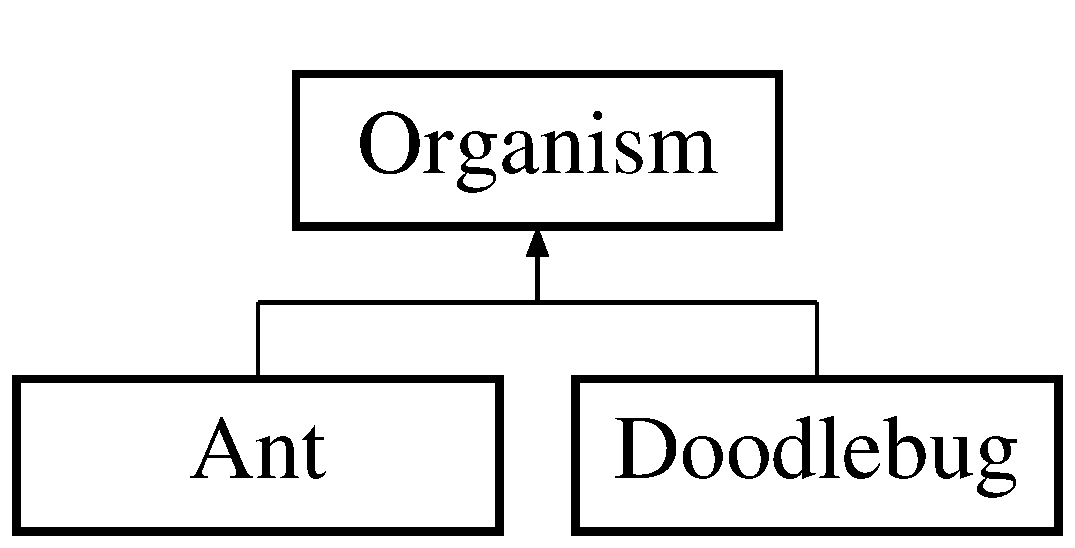
\includegraphics[height=2.000000cm]{classOrganism}
\end{center}
\end{figure}
\subsection*{Public Member Functions}
\begin{DoxyCompactItemize}
\item 
\textbf{ Organism} ()
\item 
\textbf{ Organism} (int r, int c)
\item 
\textbf{ Organism} (bool b)
\item 
bool \textbf{ is\+Prey} ()
\item 
virtual bool \textbf{ move} (\textbf{ Grid} $\ast$current)
\item 
virtual bool \textbf{ breed} (\textbf{ Grid} $\ast$current)=0
\item 
virtual bool \textbf{ eat} (\textbf{ Grid} $\ast$current)
\item 
virtual bool \textbf{ starve} ()
\item 
void \textbf{ set\+Am\+Ant} (bool b)
\item 
int \textbf{ get\+Step\+Count} ()
\item 
void \textbf{ set\+Step\+Count} (int s)
\item 
void \textbf{ set\+Column} (int c)
\item 
void \textbf{ set\+Row} (int r)
\item 
int \textbf{ get\+Row} ()
\item 
int \textbf{ get\+Column} ()
\item 
bool \textbf{ get\+Processed} ()
\item 
void \textbf{ set\+Processed} (bool set\+Processed)
\item 
virtual \textbf{ $\sim$\+Organism} ()
\end{DoxyCompactItemize}
\subsection*{Protected Attributes}
\begin{DoxyCompactItemize}
\item 
int \textbf{ row} = 0
\item 
int \textbf{ col} = 0
\item 
int \textbf{ step\+Count} = 0
\item 
bool \textbf{ am\+Ant} = false
\item 
bool \textbf{ processed} = false
\end{DoxyCompactItemize}


\subsection{Constructor \& Destructor Documentation}
\mbox{\label{classOrganism_aeb16ee24b64839584b4862384d0b53fe}} 
\index{Organism@{Organism}!Organism@{Organism}}
\index{Organism@{Organism}!Organism@{Organism}}
\subsubsection{Organism()\hspace{0.1cm}{\footnotesize\ttfamily [1/3]}}
{\footnotesize\ttfamily Organism\+::\+Organism (\begin{DoxyParamCaption}{ }\end{DoxyParamCaption})}

Function is the default constructor for an organism object that instantiates an \doxyref{Organism}{p.}{classOrganism} object. \mbox{\label{classOrganism_aa218274d783df15f6f372ba0df38decf}} 
\index{Organism@{Organism}!Organism@{Organism}}
\index{Organism@{Organism}!Organism@{Organism}}
\subsubsection{Organism()\hspace{0.1cm}{\footnotesize\ttfamily [2/3]}}
{\footnotesize\ttfamily Organism\+::\+Organism (\begin{DoxyParamCaption}\item[{int}]{r,  }\item[{int}]{c }\end{DoxyParamCaption})}

Function is another constructor for an organism object that instantiates an \doxyref{Organism}{p.}{classOrganism} object with r rows and c columns.


\begin{DoxyParams}{Parameters}
{\em r} & The row that the organism will be instantiated in. \\
\hline
{\em c} & The column that the organism will be instantiated in. \\
\hline
\end{DoxyParams}


References col, row, and step\+Count.

\mbox{\label{classOrganism_ac7d3dbebaf5df39d0a7883b2d76b4868}} 
\index{Organism@{Organism}!Organism@{Organism}}
\index{Organism@{Organism}!Organism@{Organism}}
\subsubsection{Organism()\hspace{0.1cm}{\footnotesize\ttfamily [3/3]}}
{\footnotesize\ttfamily Organism\+::\+Organism (\begin{DoxyParamCaption}\item[{bool}]{b }\end{DoxyParamCaption})}

Function is another constructor for an organism object that instantiates an \doxyref{Organism}{p.}{classOrganism} object and sets the boolean value am\+Ant to the passes in param b.


\begin{DoxyParams}{Parameters}
{\em b} & A boolean value indicating whether an organism is an ant or not. \\
\hline
\end{DoxyParams}


References am\+Ant.

\mbox{\label{classOrganism_aa5aa2e9fc3134358c929fa0c9d230c3b}} 
\index{Organism@{Organism}!````~Organism@{$\sim$\+Organism}}
\index{````~Organism@{$\sim$\+Organism}!Organism@{Organism}}
\subsubsection{$\sim$\+Organism()}
{\footnotesize\ttfamily Organism\+::$\sim$\+Organism (\begin{DoxyParamCaption}{ }\end{DoxyParamCaption})\hspace{0.3cm}{\ttfamily [virtual]}}

Function is a destructor that takes the \doxyref{Organism}{p.}{classOrganism} object and deletes it once the program is done using the object. 

\subsection{Member Function Documentation}
\mbox{\label{classOrganism_aeecced266ac9dd055a0a0caf57379fb7}} 
\index{Organism@{Organism}!breed@{breed}}
\index{breed@{breed}!Organism@{Organism}}
\subsubsection{breed()}
{\footnotesize\ttfamily virtual bool Organism\+::breed (\begin{DoxyParamCaption}\item[{\textbf{ Grid} $\ast$}]{current }\end{DoxyParamCaption})\hspace{0.3cm}{\ttfamily [pure virtual]}}



Implemented in \textbf{ Doodlebug} \doxyref{}{p.}{classDoodlebug_a6aa05cce6d3d7df55d9c3787c01fd9b2}, and \textbf{ Ant} \doxyref{}{p.}{classAnt_ab51f7167f7e9b8e942a1ca5cbcecc3ba}.



Referenced by Production\+::play\+One().

\mbox{\label{classOrganism_a8305e732b48c3a16dbc83b8a42eaa52a}} 
\index{Organism@{Organism}!eat@{eat}}
\index{eat@{eat}!Organism@{Organism}}
\subsubsection{eat()}
{\footnotesize\ttfamily bool Organism\+::eat (\begin{DoxyParamCaption}\item[{\textbf{ Grid} $\ast$}]{current }\end{DoxyParamCaption})\hspace{0.3cm}{\ttfamily [virtual]}}

Function tells whether an organism is a prey.

\begin{DoxyReturn}{Returns}
false This boolean value holds true for all organism unless ovverrided in child class. 
\end{DoxyReturn}


Reimplemented in \textbf{ Doodlebug} \doxyref{}{p.}{classDoodlebug_a00a3a3e9a9b82d6dc9affae5c4e01630}.

\mbox{\label{classOrganism_adb8661020928f339620864b6c2522e52}} 
\index{Organism@{Organism}!get\+Column@{get\+Column}}
\index{get\+Column@{get\+Column}!Organism@{Organism}}
\subsubsection{get\+Column()}
{\footnotesize\ttfamily int Organism\+::get\+Column (\begin{DoxyParamCaption}{ }\end{DoxyParamCaption})}

Function returns the current row of the organism.

\begin{DoxyReturn}{Returns}
row The current row that the organism is in. 
\end{DoxyReturn}


References col.

\mbox{\label{classOrganism_aed896c656998a22cd1d9f216c0225a61}} 
\index{Organism@{Organism}!get\+Processed@{get\+Processed}}
\index{get\+Processed@{get\+Processed}!Organism@{Organism}}
\subsubsection{get\+Processed()}
{\footnotesize\ttfamily bool Organism\+::get\+Processed (\begin{DoxyParamCaption}{ }\end{DoxyParamCaption})}

Function returns the processed status of the organism.

\begin{DoxyReturn}{Returns}
row The current processed status of the organism. 
\end{DoxyReturn}


References processed.



Referenced by Production\+::play\+One().

\mbox{\label{classOrganism_a8189241fd26884ee9c722a081f50387a}} 
\index{Organism@{Organism}!get\+Row@{get\+Row}}
\index{get\+Row@{get\+Row}!Organism@{Organism}}
\subsubsection{get\+Row()}
{\footnotesize\ttfamily int Organism\+::get\+Row (\begin{DoxyParamCaption}{ }\end{DoxyParamCaption})}

Function returns the current row of the organism.

\begin{DoxyReturn}{Returns}
row The current row that the organism is in. 
\end{DoxyReturn}


References row.

\mbox{\label{classOrganism_ab2c39f540ab6883c3038b33357d7e409}} 
\index{Organism@{Organism}!get\+Step\+Count@{get\+Step\+Count}}
\index{get\+Step\+Count@{get\+Step\+Count}!Organism@{Organism}}
\subsubsection{get\+Step\+Count()}
{\footnotesize\ttfamily int Organism\+::get\+Step\+Count (\begin{DoxyParamCaption}{ }\end{DoxyParamCaption})}

Function returns the current step\+Count of the organism.

\begin{DoxyReturn}{Returns}
step\+Count A number of steps that the organism has survived for. 
\end{DoxyReturn}


References step\+Count.



Referenced by Production\+::play\+One().

\mbox{\label{classOrganism_aa5213b2e2b0c4f227dc7dfc4c4ab411c}} 
\index{Organism@{Organism}!is\+Prey@{is\+Prey}}
\index{is\+Prey@{is\+Prey}!Organism@{Organism}}
\subsubsection{is\+Prey()}
{\footnotesize\ttfamily bool Organism\+::is\+Prey (\begin{DoxyParamCaption}{ }\end{DoxyParamCaption})}

Function tells whether an organism is a prey.

\begin{DoxyReturn}{Returns}
status A boolean value that indicates true if an organism is prey and false if the organism is not prey. 
\end{DoxyReturn}


References am\+Ant.



Referenced by Grid\+::create\+Organism().

\mbox{\label{classOrganism_ad83535a041d8cc6543a8f68c80c14122}} 
\index{Organism@{Organism}!move@{move}}
\index{move@{move}!Organism@{Organism}}
\subsubsection{move()}
{\footnotesize\ttfamily bool Organism\+::move (\begin{DoxyParamCaption}\item[{\textbf{ Grid} $\ast$}]{current }\end{DoxyParamCaption})\hspace{0.3cm}{\ttfamily [virtual]}}

Functions tells whether if the organism can move or not, and then moves it accordingly.


\begin{DoxyParams}{Parameters}
{\em current} & A pointer to the current board that the game is being played on. \\
\hline
\end{DoxyParams}
\begin{DoxyReturn}{Returns}
status A boolean value that indicates true if an ant can move and false if the ant cannot move. 
\end{DoxyReturn}


Reimplemented in \textbf{ Doodlebug} \doxyref{}{p.}{classDoodlebug_ae411913efc4e52c0f726c537dacbb778}.



References col, Grid\+::find\+Move(), Grid\+::move\+Organism(), and row.



Referenced by Tests2\+::ants\+Move\+Test(), Doodlebug\+::move(), and Production\+::play\+One().

\mbox{\label{classOrganism_aba68f4745f6b0938cf157dcd27df1868}} 
\index{Organism@{Organism}!set\+Am\+Ant@{set\+Am\+Ant}}
\index{set\+Am\+Ant@{set\+Am\+Ant}!Organism@{Organism}}
\subsubsection{set\+Am\+Ant()}
{\footnotesize\ttfamily void Organism\+::set\+Am\+Ant (\begin{DoxyParamCaption}\item[{bool}]{b }\end{DoxyParamCaption})}

Function sets the organism as an ant. 

References am\+Ant.

\mbox{\label{classOrganism_ace6498f572b31dca3a9e82c8db15d648}} 
\index{Organism@{Organism}!set\+Column@{set\+Column}}
\index{set\+Column@{set\+Column}!Organism@{Organism}}
\subsubsection{set\+Column()}
{\footnotesize\ttfamily void Organism\+::set\+Column (\begin{DoxyParamCaption}\item[{int}]{c }\end{DoxyParamCaption})}

Function sets the current row of the organism.


\begin{DoxyParams}{Parameters}
{\em r} & The given row that the organism will be in. \\
\hline
\end{DoxyParams}


References col.



Referenced by Grid\+::move\+Organism().

\mbox{\label{classOrganism_a40a6d4617337c88bda0dfeca1e053cbe}} 
\index{Organism@{Organism}!set\+Processed@{set\+Processed}}
\index{set\+Processed@{set\+Processed}!Organism@{Organism}}
\subsubsection{set\+Processed()}
{\footnotesize\ttfamily void Organism\+::set\+Processed (\begin{DoxyParamCaption}\item[{bool}]{set\+Processed }\end{DoxyParamCaption})}

Function sets the current processed status of the organism.


\begin{DoxyParams}{Parameters}
{\em set\+Processed} & A boolean value indicating what the processed status should be set to. \\
\hline
\end{DoxyParams}


References processed.



Referenced by Production\+::play\+One().

\mbox{\label{classOrganism_a8d5178cc3d41e6cf9be613f50776b233}} 
\index{Organism@{Organism}!set\+Row@{set\+Row}}
\index{set\+Row@{set\+Row}!Organism@{Organism}}
\subsubsection{set\+Row()}
{\footnotesize\ttfamily void Organism\+::set\+Row (\begin{DoxyParamCaption}\item[{int}]{r }\end{DoxyParamCaption})}

Function sets the current row of the organism.


\begin{DoxyParams}{Parameters}
{\em r} & The given row that the organism will be in. \\
\hline
\end{DoxyParams}


References row.



Referenced by Grid\+::move\+Organism().

\mbox{\label{classOrganism_a0ce8e8fc825caf906ac031907a89cdda}} 
\index{Organism@{Organism}!set\+Step\+Count@{set\+Step\+Count}}
\index{set\+Step\+Count@{set\+Step\+Count}!Organism@{Organism}}
\subsubsection{set\+Step\+Count()}
{\footnotesize\ttfamily void Organism\+::set\+Step\+Count (\begin{DoxyParamCaption}\item[{int}]{s }\end{DoxyParamCaption})}

Function sets the current step\+Count of the organism.


\begin{DoxyParams}{Parameters}
{\em s} & The given number of steps that the organism has survived for. \\
\hline
\end{DoxyParams}


References step\+Count.



Referenced by Tests2\+::ants\+Breed\+Test(), Tests2\+::doodle\+Breed\+Test(), and Production\+::play\+One().

\mbox{\label{classOrganism_ad1456a1f22de197cc74ca8cf5a1a0189}} 
\index{Organism@{Organism}!starve@{starve}}
\index{starve@{starve}!Organism@{Organism}}
\subsubsection{starve()}
{\footnotesize\ttfamily bool Organism\+::starve (\begin{DoxyParamCaption}{ }\end{DoxyParamCaption})\hspace{0.3cm}{\ttfamily [virtual]}}

Returns whether or not the organism has starved.

\begin{DoxyReturn}{Returns}
false This boolean value holds true for all organisms, unless overrided in child class. 
\end{DoxyReturn}


Reimplemented in \textbf{ Doodlebug} \doxyref{}{p.}{classDoodlebug_a7f1c26c8458f3811680c778362c0e374}.



Referenced by Production\+::play\+One().



\subsection{Field Documentation}
\mbox{\label{classOrganism_ab9742ed0a29e19e3c52ba74bdea66b51}} 
\index{Organism@{Organism}!am\+Ant@{am\+Ant}}
\index{am\+Ant@{am\+Ant}!Organism@{Organism}}
\subsubsection{am\+Ant}
{\footnotesize\ttfamily bool Organism\+::am\+Ant = false\hspace{0.3cm}{\ttfamily [protected]}}



Referenced by is\+Prey(), Organism(), and set\+Am\+Ant().

\mbox{\label{classOrganism_a8f36f6e8f707ab4bc34e5edd31bfec07}} 
\index{Organism@{Organism}!col@{col}}
\index{col@{col}!Organism@{Organism}}
\subsubsection{col}
{\footnotesize\ttfamily int Organism\+::col = 0\hspace{0.3cm}{\ttfamily [protected]}}



Referenced by Ant\+::\+Ant(), Ant\+::breed(), Doodlebug\+::breed(), Doodlebug\+::\+Doodlebug(), Doodlebug\+::eat(), get\+Column(), move(), Organism(), and set\+Column().

\mbox{\label{classOrganism_ab1d5c4cef10f9bcb16d87642c966bb4c}} 
\index{Organism@{Organism}!processed@{processed}}
\index{processed@{processed}!Organism@{Organism}}
\subsubsection{processed}
{\footnotesize\ttfamily bool Organism\+::processed = false\hspace{0.3cm}{\ttfamily [protected]}}



Referenced by get\+Processed(), and set\+Processed().

\mbox{\label{classOrganism_aa298debd9753da69e00e575f5ab2a73f}} 
\index{Organism@{Organism}!row@{row}}
\index{row@{row}!Organism@{Organism}}
\subsubsection{row}
{\footnotesize\ttfamily int Organism\+::row = 0\hspace{0.3cm}{\ttfamily [protected]}}



Referenced by Ant\+::\+Ant(), Ant\+::breed(), Doodlebug\+::breed(), Doodlebug\+::\+Doodlebug(), Doodlebug\+::eat(), get\+Row(), move(), Organism(), and set\+Row().

\mbox{\label{classOrganism_a5ebbab8a61a360037633e0d83a056e9f}} 
\index{Organism@{Organism}!step\+Count@{step\+Count}}
\index{step\+Count@{step\+Count}!Organism@{Organism}}
\subsubsection{step\+Count}
{\footnotesize\ttfamily int Organism\+::step\+Count = 0\hspace{0.3cm}{\ttfamily [protected]}}



Referenced by Ant\+::breed(), Doodlebug\+::breed(), get\+Step\+Count(), Organism(), and set\+Step\+Count().



The documentation for this class was generated from the following files\+:\begin{DoxyCompactItemize}
\item 
\textbf{ Organism.\+h}\item 
\textbf{ Organism.\+cpp}\end{DoxyCompactItemize}

\section{Production Class Reference}
\label{classProduction}\index{Production@{Production}}


{\ttfamily \#include $<$Production.\+h$>$}

\subsection*{Public Member Functions}
\begin{DoxyCompactItemize}
\item 
\textbf{ Production} (int argc, char $\ast$argv[$\,$])
\item 
bool \textbf{ run\+Production} ()
\item 
virtual \textbf{ $\sim$\+Production} ()
\item 
void \textbf{ play\+One} ()
\end{DoxyCompactItemize}
\subsection*{Private Attributes}
\begin{DoxyCompactItemize}
\item 
int \textbf{ timesteps\+Left} =1000
\item 
int \textbf{ times\+Run} = 0
\item 
int \textbf{ grid\+Size} = 20
\item 
int \textbf{ doodlebugs} = 5
\item 
int \textbf{ ants} = 100
\item 
int \textbf{ seed} = 1
\item 
int \textbf{ pause} = 0
\item 
\textbf{ Grid} $\ast$ \textbf{ board}
\item 
int \textbf{ new\+Ants} = 0
\item 
int \textbf{ new\+Doodlebugs} = 0
\item 
int \textbf{ remaining\+Ants} = 0
\item 
int \textbf{ remaining\+Doodlebugs} = 0
\end{DoxyCompactItemize}


\subsection{Constructor \& Destructor Documentation}
\mbox{\label{classProduction_a24439558b7672feaea80dc0ab1b53ff2}} 
\index{Production@{Production}!Production@{Production}}
\index{Production@{Production}!Production@{Production}}
\subsubsection{Production()}
{\footnotesize\ttfamily Production\+::\+Production (\begin{DoxyParamCaption}\item[{int}]{argc,  }\item[{char $\ast$}]{argv[$\,$] }\end{DoxyParamCaption})}

Function is the default constructor for a production object that instantiates \doxyref{Production}{p.}{classProduction} object, and sets the timestepsleft to 100. 
\begin{DoxyParams}{Parameters}
{\em argc} & Number of words on the command line \\
\hline
{\em argv} & Array of pointers to character strings representing the words on the command line. \\
\hline
\end{DoxyParams}


References ant, ants, board, doodlebug, doodlebugs, empty, Grid\+::get\+Cell\+Occupant(), grid\+Size, pause, Grid\+::print\+Grid(), seed, Grid\+::set\+Cell\+Occupant(), Grid\+::set\+Cell\+Organism(), and timesteps\+Left.



Referenced by main().

\mbox{\label{classProduction_ab5b3060f9e0a2bc189844e426d693dab}} 
\index{Production@{Production}!````~Production@{$\sim$\+Production}}
\index{````~Production@{$\sim$\+Production}!Production@{Production}}
\subsubsection{$\sim$\+Production()}
{\footnotesize\ttfamily Production\+::$\sim$\+Production (\begin{DoxyParamCaption}{ }\end{DoxyParamCaption})\hspace{0.3cm}{\ttfamily [virtual]}}

Function is a destructor that takes the production object and deletes it once the program is done using the object. 

Referenced by main().



\subsection{Member Function Documentation}
\mbox{\label{classProduction_a4948eadf0b30dcc30d02fa9be98d9f6b}} 
\index{Production@{Production}!play\+One@{play\+One}}
\index{play\+One@{play\+One}!Production@{Production}}
\subsubsection{play\+One()}
{\footnotesize\ttfamily void Production\+::play\+One (\begin{DoxyParamCaption}{ }\end{DoxyParamCaption})}

Runs through one iteration of the game. 

References ant, board, Organism\+::breed(), Grid\+::delete\+Organism(), doodlebug, Grid\+::get\+Cell\+Occupant(), Grid\+::get\+Cell\+Organism(), Organism\+::get\+Processed(), Organism\+::get\+Step\+Count(), grid\+Size, Organism\+::move(), new\+Ants, new\+Doodlebugs, Organism\+::set\+Processed(), Organism\+::set\+Step\+Count(), Organism\+::starve(), and times\+Run.



Referenced by run\+Production().

\mbox{\label{classProduction_a1d66853eafae2580089eff44f12f07ba}} 
\index{Production@{Production}!run\+Production@{run\+Production}}
\index{run\+Production@{run\+Production}!Production@{Production}}
\subsubsection{run\+Production()}
{\footnotesize\ttfamily bool Production\+::run\+Production (\begin{DoxyParamCaption}{ }\end{DoxyParamCaption})}

Function that runs the production while there are still time steps left.

\begin{DoxyReturn}{Returns}
result A boolean value true if the production was able to run successfully, and false if the production was not able to run successfully. 
\end{DoxyReturn}


References ant, ants, board, doodlebug, doodlebugs, Grid\+::get\+Cell\+Occupant(), grid\+Size, new\+Ants, new\+Doodlebugs, pause, play\+One(), Grid\+::print\+Grid(), remaining\+Ants, remaining\+Doodlebugs, seed, times\+Run, and timesteps\+Left.



Referenced by main().



\subsection{Field Documentation}
\mbox{\label{classProduction_aba80c58c0a9aeb31f0b771465695275d}} 
\index{Production@{Production}!ants@{ants}}
\index{ants@{ants}!Production@{Production}}
\subsubsection{ants}
{\footnotesize\ttfamily int Production\+::ants = 100\hspace{0.3cm}{\ttfamily [private]}}



Referenced by Production(), and run\+Production().

\mbox{\label{classProduction_ab8408abba9ecd29ccb8e1706ff43c0fc}} 
\index{Production@{Production}!board@{board}}
\index{board@{board}!Production@{Production}}
\subsubsection{board}
{\footnotesize\ttfamily \textbf{ Grid}$\ast$ Production\+::board\hspace{0.3cm}{\ttfamily [private]}}



Referenced by play\+One(), Production(), and run\+Production().

\mbox{\label{classProduction_ac91f33eade84867c82cfb7ad2a1bf77a}} 
\index{Production@{Production}!doodlebugs@{doodlebugs}}
\index{doodlebugs@{doodlebugs}!Production@{Production}}
\subsubsection{doodlebugs}
{\footnotesize\ttfamily int Production\+::doodlebugs = 5\hspace{0.3cm}{\ttfamily [private]}}



Referenced by Production(), and run\+Production().

\mbox{\label{classProduction_aec26b656d2e7519d1a1898810bd1c0da}} 
\index{Production@{Production}!grid\+Size@{grid\+Size}}
\index{grid\+Size@{grid\+Size}!Production@{Production}}
\subsubsection{grid\+Size}
{\footnotesize\ttfamily int Production\+::grid\+Size = 20\hspace{0.3cm}{\ttfamily [private]}}



Referenced by play\+One(), Production(), and run\+Production().

\mbox{\label{classProduction_a2b06ca154b0c1849f2c402e174715674}} 
\index{Production@{Production}!new\+Ants@{new\+Ants}}
\index{new\+Ants@{new\+Ants}!Production@{Production}}
\subsubsection{new\+Ants}
{\footnotesize\ttfamily int Production\+::new\+Ants = 0\hspace{0.3cm}{\ttfamily [private]}}



Referenced by play\+One(), and run\+Production().

\mbox{\label{classProduction_a4d600fde47dc7c71f9339e983947bfaf}} 
\index{Production@{Production}!new\+Doodlebugs@{new\+Doodlebugs}}
\index{new\+Doodlebugs@{new\+Doodlebugs}!Production@{Production}}
\subsubsection{new\+Doodlebugs}
{\footnotesize\ttfamily int Production\+::new\+Doodlebugs = 0\hspace{0.3cm}{\ttfamily [private]}}



Referenced by play\+One(), and run\+Production().

\mbox{\label{classProduction_af570feb7415a4d5b1a9176dacd9d6b64}} 
\index{Production@{Production}!pause@{pause}}
\index{pause@{pause}!Production@{Production}}
\subsubsection{pause}
{\footnotesize\ttfamily int Production\+::pause = 0\hspace{0.3cm}{\ttfamily [private]}}



Referenced by Production(), and run\+Production().

\mbox{\label{classProduction_aabb1ccc17955b39a7bd5e12c60ded94c}} 
\index{Production@{Production}!remaining\+Ants@{remaining\+Ants}}
\index{remaining\+Ants@{remaining\+Ants}!Production@{Production}}
\subsubsection{remaining\+Ants}
{\footnotesize\ttfamily int Production\+::remaining\+Ants = 0\hspace{0.3cm}{\ttfamily [private]}}



Referenced by run\+Production().

\mbox{\label{classProduction_a36dd357cae048fb1d8266212362d52dd}} 
\index{Production@{Production}!remaining\+Doodlebugs@{remaining\+Doodlebugs}}
\index{remaining\+Doodlebugs@{remaining\+Doodlebugs}!Production@{Production}}
\subsubsection{remaining\+Doodlebugs}
{\footnotesize\ttfamily int Production\+::remaining\+Doodlebugs = 0\hspace{0.3cm}{\ttfamily [private]}}



Referenced by run\+Production().

\mbox{\label{classProduction_adb474287b0143fccb9d440ccc54ba624}} 
\index{Production@{Production}!seed@{seed}}
\index{seed@{seed}!Production@{Production}}
\subsubsection{seed}
{\footnotesize\ttfamily int Production\+::seed = 1\hspace{0.3cm}{\ttfamily [private]}}



Referenced by Production(), and run\+Production().

\mbox{\label{classProduction_a7634272460cb1dbf7c45d1d306551542}} 
\index{Production@{Production}!times\+Run@{times\+Run}}
\index{times\+Run@{times\+Run}!Production@{Production}}
\subsubsection{times\+Run}
{\footnotesize\ttfamily int Production\+::times\+Run = 0\hspace{0.3cm}{\ttfamily [private]}}



Referenced by play\+One(), and run\+Production().

\mbox{\label{classProduction_a5fcf03b482712c458184ae4fd3f8e461}} 
\index{Production@{Production}!timesteps\+Left@{timesteps\+Left}}
\index{timesteps\+Left@{timesteps\+Left}!Production@{Production}}
\subsubsection{timesteps\+Left}
{\footnotesize\ttfamily int Production\+::timesteps\+Left =1000\hspace{0.3cm}{\ttfamily [private]}}



Referenced by Production(), and run\+Production().



The documentation for this class was generated from the following files\+:\begin{DoxyCompactItemize}
\item 
\textbf{ Production.\+h}\item 
\textbf{ Production.\+cpp}\end{DoxyCompactItemize}

\section{Tests2 Class Reference}
\label{classTests2}\index{Tests2@{Tests2}}


{\ttfamily \#include $<$Tests2.\+h$>$}

\subsection*{Public Member Functions}
\begin{DoxyCompactItemize}
\item 
\textbf{ Tests2} ()
\item 
bool \textbf{ do\+Tests} ()
\item 
bool \textbf{ grid\+Test} ()
\item 
bool \textbf{ make\+Ants\+Test} ()
\item 
bool \textbf{ ants\+Move\+Test} ()
\item 
bool \textbf{ ants\+Breed\+Test} ()
\item 
bool \textbf{ ants\+Die\+Test} ()
\item 
bool \textbf{ make\+Doodles\+Test} ()
\item 
bool \textbf{ doodle\+Move\+Test} ()
\item 
bool \textbf{ doodle\+Breed\+Test} ()
\item 
bool \textbf{ doodle\+Eat\+Test} ()
\item 
bool \textbf{ doodle\+Dietest} ()
\item 
bool \textbf{ cell\+Occupant\+Organism\+Tests} ()
\item 
bool \textbf{ check\+Neighbors\+Test} ()
\item 
bool \textbf{ find\+Food\+Test} ()
\item 
bool \textbf{ find\+Move\+Test} ()
\item 
bool \textbf{ move\+Organism\+Test} ()
\item 
bool \textbf{ print\+Grid\+And\+Cell\+Test} ()
\item 
virtual \textbf{ $\sim$\+Tests2} ()
\end{DoxyCompactItemize}


\subsection{Constructor \& Destructor Documentation}
\mbox{\label{classTests2_a6d7d8d248dd3d544199769baa1face60}} 
\index{Tests2@{Tests2}!Tests2@{Tests2}}
\index{Tests2@{Tests2}!Tests2@{Tests2}}
\subsubsection{Tests2()}
{\footnotesize\ttfamily Tests2\+::\+Tests2 (\begin{DoxyParamCaption}{ }\end{DoxyParamCaption})}

Function is the default constructor for a test object that instantiates an test object. \mbox{\label{classTests2_abed1a850ef511b7c06ae418cb3bbd5d9}} 
\index{Tests2@{Tests2}!````~Tests2@{$\sim$\+Tests2}}
\index{````~Tests2@{$\sim$\+Tests2}!Tests2@{Tests2}}
\subsubsection{$\sim$\+Tests2()}
{\footnotesize\ttfamily Tests2\+::$\sim$\+Tests2 (\begin{DoxyParamCaption}{ }\end{DoxyParamCaption})\hspace{0.3cm}{\ttfamily [virtual]}}

Function is a destructor that takes the Test object and deletes it once the program is done using the object. 

Referenced by main().



\subsection{Member Function Documentation}
\mbox{\label{classTests2_a21e7692afbdfb694caf370670cbeb7d4}} 
\index{Tests2@{Tests2}!ants\+Breed\+Test@{ants\+Breed\+Test}}
\index{ants\+Breed\+Test@{ants\+Breed\+Test}!Tests2@{Tests2}}
\subsubsection{ants\+Breed\+Test()}
{\footnotesize\ttfamily bool Tests2\+::ants\+Breed\+Test (\begin{DoxyParamCaption}{ }\end{DoxyParamCaption})}

Function calls the ants\+Breed\+Test and returns true if tests pass.

\begin{DoxyReturn}{Returns}
result true if the tests were puts(\char`\"{}\+Printing grid after.\char`\"{}); my\+Grid\+\_\+p-\/$>$print\+Grid();able to pass and false if they were not able to pass. 
\end{DoxyReturn}


References ant, Ant\+::breed(), empty, Grid\+::get\+Cell\+Occupant(), Grid\+::print\+Grid(), Grid\+::set\+Cell\+Occupant(), Grid\+::set\+Cell\+Organism(), and Organism\+::set\+Step\+Count().



Referenced by do\+Tests().

\mbox{\label{classTests2_a045d58417814d72bcf4c97b2ebb51461}} 
\index{Tests2@{Tests2}!ants\+Die\+Test@{ants\+Die\+Test}}
\index{ants\+Die\+Test@{ants\+Die\+Test}!Tests2@{Tests2}}
\subsubsection{ants\+Die\+Test()}
{\footnotesize\ttfamily bool Tests2\+::ants\+Die\+Test (\begin{DoxyParamCaption}{ }\end{DoxyParamCaption})}

Function calls the ants\+Die\+Test and returns true if tests pass.

\begin{DoxyReturn}{Returns}
result true if the tests were able to pass and false if they were not able to pass. 
\end{DoxyReturn}


References ant, doodlebug, Doodlebug\+::eat(), Grid\+::get\+Cell\+Occupant(), Grid\+::print\+Grid(), Grid\+::set\+Cell\+Occupant(), and Grid\+::set\+Cell\+Organism().



Referenced by do\+Tests().

\mbox{\label{classTests2_a7694d2797eba6fadc40234d527f6afbe}} 
\index{Tests2@{Tests2}!ants\+Move\+Test@{ants\+Move\+Test}}
\index{ants\+Move\+Test@{ants\+Move\+Test}!Tests2@{Tests2}}
\subsubsection{ants\+Move\+Test()}
{\footnotesize\ttfamily bool Tests2\+::ants\+Move\+Test (\begin{DoxyParamCaption}{ }\end{DoxyParamCaption})}

Function calls the ants\+Movetest and returns true if tests pass.

\begin{DoxyReturn}{Returns}
result true if the tests were able to pass and false if they were not able to pass. 
\end{DoxyReturn}


References ant, empty, Grid\+::get\+Cell\+Occupant(), Organism\+::move(), Grid\+::print\+Grid(), Grid\+::set\+Cell\+Occupant(), and Grid\+::set\+Cell\+Organism().



Referenced by do\+Tests().

\mbox{\label{classTests2_a9ba51b5a047d1f970aa50b1c3f07c650}} 
\index{Tests2@{Tests2}!cell\+Occupant\+Organism\+Tests@{cell\+Occupant\+Organism\+Tests}}
\index{cell\+Occupant\+Organism\+Tests@{cell\+Occupant\+Organism\+Tests}!Tests2@{Tests2}}
\subsubsection{cell\+Occupant\+Organism\+Tests()}
{\footnotesize\ttfamily bool Tests2\+::cell\+Occupant\+Organism\+Tests (\begin{DoxyParamCaption}{ }\end{DoxyParamCaption})}



References ant, Grid\+::delete\+Organism(), doodlebug, empty, Grid\+::get\+Cell\+Occupant(), Grid\+::get\+Cell\+Organism(), Grid\+::print\+Grid(), Grid\+::set\+Cell\+Occupant(), and Grid\+::set\+Cell\+Organism().



Referenced by do\+Tests().

\mbox{\label{classTests2_ad48c21e18b306f9e54a261f9778e649f}} 
\index{Tests2@{Tests2}!check\+Neighbors\+Test@{check\+Neighbors\+Test}}
\index{check\+Neighbors\+Test@{check\+Neighbors\+Test}!Tests2@{Tests2}}
\subsubsection{check\+Neighbors\+Test()}
{\footnotesize\ttfamily bool Tests2\+::check\+Neighbors\+Test (\begin{DoxyParamCaption}{ }\end{DoxyParamCaption})}

Function calls the check\+Neighbors\+Test and returns true if tests pass.

\begin{DoxyReturn}{Returns}
result true if the tests were able to pass and false if they were not able to pass. 
\end{DoxyReturn}


References ant, Grid\+::check\+Neighbors(), empty, Grid\+::print\+Grid(), Grid\+::set\+Cell\+Occupant(), Grid\+::set\+Cell\+Organism(), and unavailable.



Referenced by do\+Tests().

\mbox{\label{classTests2_a317dc926bf93038f188c999df7a85682}} 
\index{Tests2@{Tests2}!doodle\+Breed\+Test@{doodle\+Breed\+Test}}
\index{doodle\+Breed\+Test@{doodle\+Breed\+Test}!Tests2@{Tests2}}
\subsubsection{doodle\+Breed\+Test()}
{\footnotesize\ttfamily bool Tests2\+::doodle\+Breed\+Test (\begin{DoxyParamCaption}{ }\end{DoxyParamCaption})}

Function calls the doodle\+Breed\+Test and returns true if tests pass.

\begin{DoxyReturn}{Returns}
result true if the tests were able to pass and false if they were not able to pass. 
\end{DoxyReturn}


References Doodlebug\+::breed(), doodlebug, empty, Grid\+::get\+Cell\+Occupant(), Grid\+::print\+Grid(), Grid\+::set\+Cell\+Occupant(), Grid\+::set\+Cell\+Organism(), and Organism\+::set\+Step\+Count().



Referenced by do\+Tests().

\mbox{\label{classTests2_aaf403f9bb7338771173e2053ea4f95fc}} 
\index{Tests2@{Tests2}!doodle\+Dietest@{doodle\+Dietest}}
\index{doodle\+Dietest@{doodle\+Dietest}!Tests2@{Tests2}}
\subsubsection{doodle\+Dietest()}
{\footnotesize\ttfamily bool Tests2\+::doodle\+Dietest (\begin{DoxyParamCaption}{ }\end{DoxyParamCaption})}

Function calls the doodle\+Dietest and returns true if tests pass.

\begin{DoxyReturn}{Returns}
result true if the tests were able to pass and false if they were not able to pass. 
\end{DoxyReturn}


Referenced by do\+Tests().

\mbox{\label{classTests2_ae35f30e7d95e581cc4ce1316409c71ac}} 
\index{Tests2@{Tests2}!doodle\+Eat\+Test@{doodle\+Eat\+Test}}
\index{doodle\+Eat\+Test@{doodle\+Eat\+Test}!Tests2@{Tests2}}
\subsubsection{doodle\+Eat\+Test()}
{\footnotesize\ttfamily bool Tests2\+::doodle\+Eat\+Test (\begin{DoxyParamCaption}{ }\end{DoxyParamCaption})}

Function calls the doodle\+Eat\+Test and returns true if tests pass.

\begin{DoxyReturn}{Returns}
result true if the tests were able to pass and false if they were not able to pass. 
\end{DoxyReturn}


References ant, doodlebug, Doodlebug\+::eat(), Grid\+::get\+Cell\+Occupant(), Grid\+::print\+Grid(), Grid\+::set\+Cell\+Occupant(), and Grid\+::set\+Cell\+Organism().



Referenced by do\+Tests().

\mbox{\label{classTests2_a2143f2192836626e7214d37b504df381}} 
\index{Tests2@{Tests2}!doodle\+Move\+Test@{doodle\+Move\+Test}}
\index{doodle\+Move\+Test@{doodle\+Move\+Test}!Tests2@{Tests2}}
\subsubsection{doodle\+Move\+Test()}
{\footnotesize\ttfamily bool Tests2\+::doodle\+Move\+Test (\begin{DoxyParamCaption}{ }\end{DoxyParamCaption})}

Function calls the doodle\+Move\+Test and returns true if tests pass.

\begin{DoxyReturn}{Returns}
result true if the tests were able to pass and false if they were not able to pass. 
\end{DoxyReturn}


References doodlebug, Grid\+::get\+Cell\+Occupant(), Doodlebug\+::move(), Grid\+::set\+Cell\+Occupant(), and Grid\+::set\+Cell\+Organism().



Referenced by do\+Tests().

\mbox{\label{classTests2_a7392382310966597d685c8aa3a4a2f88}} 
\index{Tests2@{Tests2}!do\+Tests@{do\+Tests}}
\index{do\+Tests@{do\+Tests}!Tests2@{Tests2}}
\subsubsection{do\+Tests()}
{\footnotesize\ttfamily bool Tests2\+::do\+Tests (\begin{DoxyParamCaption}{ }\end{DoxyParamCaption})}

Function calls all of the test functions and returns a boolean value that indicates whether or not all the tests passed or not.

\begin{DoxyReturn}{Returns}
results A boolean value that reads true if all of the tests passed and false if any of the tests fail. 
\end{DoxyReturn}


References ants\+Breed\+Test(), ants\+Die\+Test(), ants\+Move\+Test(), cell\+Occupant\+Organism\+Tests(), check\+Neighbors\+Test(), doodle\+Breed\+Test(), doodle\+Dietest(), doodle\+Eat\+Test(), doodle\+Move\+Test(), find\+Food\+Test(), find\+Move\+Test(), grid\+Test(), make\+Ants\+Test(), make\+Doodles\+Test(), move\+Organism\+Test(), and print\+Grid\+And\+Cell\+Test().



Referenced by main().

\mbox{\label{classTests2_a29f005f11c9771786d1dd969aea9b051}} 
\index{Tests2@{Tests2}!find\+Food\+Test@{find\+Food\+Test}}
\index{find\+Food\+Test@{find\+Food\+Test}!Tests2@{Tests2}}
\subsubsection{find\+Food\+Test()}
{\footnotesize\ttfamily bool Tests2\+::find\+Food\+Test (\begin{DoxyParamCaption}{ }\end{DoxyParamCaption})}

Function calls the find\+Food\+Test and returns true if tests pass.

\begin{DoxyReturn}{Returns}
result true if the tests were able to pass and false if they were not able to pass. 
\end{DoxyReturn}


References ant, doodlebug, Grid\+::find\+Food(), Grid\+::print\+Grid(), Grid\+::set\+Cell\+Occupant(), and Grid\+::set\+Cell\+Organism().



Referenced by do\+Tests().

\mbox{\label{classTests2_af2a95558f0f9cd28a89c82324576ad2e}} 
\index{Tests2@{Tests2}!find\+Move\+Test@{find\+Move\+Test}}
\index{find\+Move\+Test@{find\+Move\+Test}!Tests2@{Tests2}}
\subsubsection{find\+Move\+Test()}
{\footnotesize\ttfamily bool Tests2\+::find\+Move\+Test (\begin{DoxyParamCaption}{ }\end{DoxyParamCaption})}

Function calls the find\+Move\+Test and returns true if tests pass.

\begin{DoxyReturn}{Returns}
result true if the tests were able to pass and false if they were not able to pass. 
\end{DoxyReturn}


References ant, doodlebug, Grid\+::find\+Move(), Grid\+::print\+Grid(), Grid\+::set\+Cell\+Occupant(), and Grid\+::set\+Cell\+Organism().



Referenced by do\+Tests().

\mbox{\label{classTests2_afe90de3a79c4105e63205cb8f019bbb2}} 
\index{Tests2@{Tests2}!grid\+Test@{grid\+Test}}
\index{grid\+Test@{grid\+Test}!Tests2@{Tests2}}
\subsubsection{grid\+Test()}
{\footnotesize\ttfamily bool Tests2\+::grid\+Test (\begin{DoxyParamCaption}{ }\end{DoxyParamCaption})}

Function calls the grid object and checks whether the grid was instantiated correctly and if the grid sets the occupancy statuses correctly.

\begin{DoxyReturn}{Returns}
results A boolean value that reads true if the the grid was able to set the cell occupancy statuses correctly. 
\end{DoxyReturn}


References ant, empty, Grid\+::get\+Cell\+Occupant(), Grid\+::set\+Cell\+Occupant(), and Grid\+::$\sim$\+Grid().



Referenced by do\+Tests().

\mbox{\label{classTests2_aa4d40396194cf770aa82dc11b449ea62}} 
\index{Tests2@{Tests2}!make\+Ants\+Test@{make\+Ants\+Test}}
\index{make\+Ants\+Test@{make\+Ants\+Test}!Tests2@{Tests2}}
\subsubsection{make\+Ants\+Test()}
{\footnotesize\ttfamily bool Tests2\+::make\+Ants\+Test (\begin{DoxyParamCaption}{ }\end{DoxyParamCaption})}

Function checks if the ant object were able to be instantiate correctly and if the occupancy status was set correctly.

\begin{DoxyReturn}{Returns}
result A boolean value that is true if the ant object was instantiated correctly and if its occupancy status was set to ant, and false if this was not done. 
\end{DoxyReturn}


References ant, doodlebug, empty, Grid\+::get\+Cell\+Occupant(), Grid\+::print\+Grid(), and Grid\+::set\+Cell\+Occupant().



Referenced by do\+Tests().

\mbox{\label{classTests2_a0c6c7e5d60e7c6dc8799fa14e2b997b4}} 
\index{Tests2@{Tests2}!make\+Doodles\+Test@{make\+Doodles\+Test}}
\index{make\+Doodles\+Test@{make\+Doodles\+Test}!Tests2@{Tests2}}
\subsubsection{make\+Doodles\+Test()}
{\footnotesize\ttfamily bool Tests2\+::make\+Doodles\+Test (\begin{DoxyParamCaption}{ }\end{DoxyParamCaption})}

Function calls the make\+Doodles\+Test and returns true if tests pass.

\begin{DoxyReturn}{Returns}
result true if the tests were able to pass and false if they were not able to pass. 
\end{DoxyReturn}


Referenced by do\+Tests().

\mbox{\label{classTests2_a2ab8e952ccdd1777f6d549ad9409e61b}} 
\index{Tests2@{Tests2}!move\+Organism\+Test@{move\+Organism\+Test}}
\index{move\+Organism\+Test@{move\+Organism\+Test}!Tests2@{Tests2}}
\subsubsection{move\+Organism\+Test()}
{\footnotesize\ttfamily bool Tests2\+::move\+Organism\+Test (\begin{DoxyParamCaption}{ }\end{DoxyParamCaption})}

Function calls the move\+Organism\+Test and returns true if tests pass.

\begin{DoxyReturn}{Returns}
result true if the tests were able to pass and false if they were not able to pass. 
\end{DoxyReturn}


References ant, doodlebug, empty, Grid\+::get\+Cell\+Occupant(), Grid\+::move\+Organism(), Grid\+::print\+Grid(), Grid\+::set\+Cell\+Occupant(), and Grid\+::set\+Cell\+Organism().



Referenced by do\+Tests().

\mbox{\label{classTests2_a5c27bd3a353488311cbc4323d34baa00}} 
\index{Tests2@{Tests2}!print\+Grid\+And\+Cell\+Test@{print\+Grid\+And\+Cell\+Test}}
\index{print\+Grid\+And\+Cell\+Test@{print\+Grid\+And\+Cell\+Test}!Tests2@{Tests2}}
\subsubsection{print\+Grid\+And\+Cell\+Test()}
{\footnotesize\ttfamily bool Tests2\+::print\+Grid\+And\+Cell\+Test (\begin{DoxyParamCaption}{ }\end{DoxyParamCaption})}

Function calls the print\+Grid\+Test and the print\+Cell\+Test and returns true if tests pass.

\begin{DoxyReturn}{Returns}
result true if the tests were able to pass and false if they were not able to pass. 
\end{DoxyReturn}


References ant, doodlebug, Grid\+::get\+Cell(), Cell\+::print\+Cell(), Grid\+::print\+Grid(), Grid\+::set\+Cell\+Occupant(), and Grid\+::set\+Cell\+Organism().



Referenced by do\+Tests().



The documentation for this class was generated from the following files\+:\begin{DoxyCompactItemize}
\item 
\textbf{ Tests2.\+h}\item 
\textbf{ Tests2.\+cpp}\end{DoxyCompactItemize}

\chapter{File Documentation}
\section{Ant.\+cpp File Reference}
\label{Ant_8cpp}\index{Ant.\+cpp@{Ant.\+cpp}}
{\ttfamily \#include \char`\"{}Ant.\+h\char`\"{}}\newline
{\ttfamily \#include $<$stdlib.\+h$>$}\newline
{\ttfamily \#include $<$stdio.\+h$>$}\newline

\section{Ant.\+h File Reference}
\label{Ant_8h}\index{Ant.\+h@{Ant.\+h}}
{\ttfamily \#include \char`\"{}Organism.\+h\char`\"{}}\newline
\subsection*{Data Structures}
\begin{DoxyCompactItemize}
\item 
class \textbf{ Ant}
\end{DoxyCompactItemize}

\section{Ants\+And\+Doodles.\+cpp File Reference}
\label{AntsAndDoodles_8cpp}\index{Ants\+And\+Doodles.\+cpp@{Ants\+And\+Doodles.\+cpp}}
{\ttfamily \#include $<$iostream$>$}\newline
{\ttfamily \#include \char`\"{}Tests2.\+h\char`\"{}}\newline
{\ttfamily \#include \char`\"{}Production.\+h\char`\"{}}\newline
\subsection*{Functions}
\begin{DoxyCompactItemize}
\item 
int \textbf{ main} (int argc, char $\ast$argv[$\,$])
\end{DoxyCompactItemize}


\subsection{Function Documentation}
\mbox{\label{AntsAndDoodles_8cpp_a0ddf1224851353fc92bfbff6f499fa97}} 
\index{Ants\+And\+Doodles.\+cpp@{Ants\+And\+Doodles.\+cpp}!main@{main}}
\index{main@{main}!Ants\+And\+Doodles.\+cpp@{Ants\+And\+Doodles.\+cpp}}
\subsubsection{main()}
{\footnotesize\ttfamily int main (\begin{DoxyParamCaption}\item[{int}]{argc,  }\item[{char $\ast$}]{argv[$\,$] }\end{DoxyParamCaption})}

The main function that calls production and checks to see if it is working properly.


\begin{DoxyParams}{Parameters}
{\em argc} & Number of words on the command line \\
\hline
{\em argv} & Array of pointers to character strings representing the words on the command line. \\
\hline
\end{DoxyParams}
\begin{DoxyReturn}{Returns}
true if Program was able to play ants and doodle bugs false if something went wrong in the tests. 
\end{DoxyReturn}


References Tests2\+::do\+Tests(), Production\+::\+Production(), Production\+::run\+Production(), Production\+::$\sim$\+Production(), and Tests2\+::$\sim$\+Tests2().


\section{Cell.\+cpp File Reference}
\label{Cell_8cpp}\index{Cell.\+cpp@{Cell.\+cpp}}
{\ttfamily \#include \char`\"{}Cell.\+h\char`\"{}}\newline
{\ttfamily \#include $<$stdio.\+h$>$}\newline

\section{Cell.\+h File Reference}
\label{Cell_8h}\index{Cell.\+h@{Cell.\+h}}
\subsection*{Data Structures}
\begin{DoxyCompactItemize}
\item 
class \textbf{ Cell}
\end{DoxyCompactItemize}
\subsection*{Enumerations}
\begin{DoxyCompactItemize}
\item 
enum \textbf{ occupation\+Status} \{ \textbf{ empty}, 
\textbf{ ant}, 
\textbf{ doodlebug}, 
\textbf{ unavailable}
 \}
\end{DoxyCompactItemize}


\subsection{Enumeration Type Documentation}
\mbox{\label{Cell_8h_abcce8bf608a2504bf718b7234aa15acb}} 
\index{Cell.\+h@{Cell.\+h}!occupation\+Status@{occupation\+Status}}
\index{occupation\+Status@{occupation\+Status}!Cell.\+h@{Cell.\+h}}
\subsubsection{occupation\+Status}
{\footnotesize\ttfamily enum \textbf{ occupation\+Status}}

\begin{DoxyEnumFields}{Enumerator}
\raisebox{\heightof{T}}[0pt][0pt]{\index{empty@{empty}!Cell.\+h@{Cell.\+h}}\index{Cell.\+h@{Cell.\+h}!empty@{empty}}}\mbox{\label{Cell_8h_abcce8bf608a2504bf718b7234aa15acbae8654263bd8adf1d0922f427d8f3fc1b}} 
empty&\\
\hline

\raisebox{\heightof{T}}[0pt][0pt]{\index{ant@{ant}!Cell.\+h@{Cell.\+h}}\index{Cell.\+h@{Cell.\+h}!ant@{ant}}}\mbox{\label{Cell_8h_abcce8bf608a2504bf718b7234aa15acbacc8f2f9c5b15a05a2f336152b3794aa9}} 
ant&\\
\hline

\raisebox{\heightof{T}}[0pt][0pt]{\index{doodlebug@{doodlebug}!Cell.\+h@{Cell.\+h}}\index{Cell.\+h@{Cell.\+h}!doodlebug@{doodlebug}}}\mbox{\label{Cell_8h_abcce8bf608a2504bf718b7234aa15acba55f311222a925986c2589e11b469c0f2}} 
doodlebug&\\
\hline

\raisebox{\heightof{T}}[0pt][0pt]{\index{unavailable@{unavailable}!Cell.\+h@{Cell.\+h}}\index{Cell.\+h@{Cell.\+h}!unavailable@{unavailable}}}\mbox{\label{Cell_8h_abcce8bf608a2504bf718b7234aa15acba048ba3a1fc805129c1d963377f33aab2}} 
unavailable&\\
\hline

\end{DoxyEnumFields}

\section{Doodlebug.\+cpp File Reference}
\label{Doodlebug_8cpp}\index{Doodlebug.\+cpp@{Doodlebug.\+cpp}}
{\ttfamily \#include \char`\"{}Doodlebug.\+h\char`\"{}}\newline
{\ttfamily \#include $<$stdlib.\+h$>$}\newline
{\ttfamily \#include $<$stdio.\+h$>$}\newline

\section{Doodlebug.\+h File Reference}
\label{Doodlebug_8h}\index{Doodlebug.\+h@{Doodlebug.\+h}}
{\ttfamily \#include \char`\"{}Organism.\+h\char`\"{}}\newline
\subsection*{Data Structures}
\begin{DoxyCompactItemize}
\item 
class \textbf{ Doodlebug}
\end{DoxyCompactItemize}

\section{Grid.\+cpp File Reference}
\label{Grid_8cpp}\index{Grid.\+cpp@{Grid.\+cpp}}
{\ttfamily \#include $<$iostream$>$}\newline
{\ttfamily \#include $<$iomanip$>$}\newline
{\ttfamily \#include \char`\"{}Grid.\+h\char`\"{}}\newline
{\ttfamily \#include \char`\"{}Cell.\+h\char`\"{}}\newline
{\ttfamily \#include \char`\"{}Organism.\+h\char`\"{}}\newline
{\ttfamily \#include \char`\"{}Ant.\+h\char`\"{}}\newline
{\ttfamily \#include \char`\"{}Doodlebug.\+h\char`\"{}}\newline

\section{Grid.\+h File Reference}
\label{Grid_8h}\index{Grid.\+h@{Grid.\+h}}
{\ttfamily \#include \char`\"{}Cell.\+h\char`\"{}}\newline
\subsection*{Data Structures}
\begin{DoxyCompactItemize}
\item 
class \textbf{ Grid}
\end{DoxyCompactItemize}

\section{Organism.\+cpp File Reference}
\label{Organism_8cpp}\index{Organism.\+cpp@{Organism.\+cpp}}
{\ttfamily \#include \char`\"{}Organism.\+h\char`\"{}}\newline
{\ttfamily \#include \char`\"{}Grid.\+h\char`\"{}}\newline
{\ttfamily \#include $<$stdlib.\+h$>$}\newline
{\ttfamily \#include $<$stdio.\+h$>$}\newline

\section{Organism.\+h File Reference}
\label{Organism_8h}\index{Organism.\+h@{Organism.\+h}}
{\ttfamily \#include \char`\"{}Grid.\+h\char`\"{}}\newline
\subsection*{Data Structures}
\begin{DoxyCompactItemize}
\item 
class \textbf{ Organism}
\end{DoxyCompactItemize}

\section{Production.\+cpp File Reference}
\label{Production_8cpp}\index{Production.\+cpp@{Production.\+cpp}}
{\ttfamily \#include \char`\"{}Production.\+h\char`\"{}}\newline
{\ttfamily \#include $<$stdio.\+h$>$}\newline
{\ttfamily \#include $<$stdlib.\+h$>$}\newline
{\ttfamily \#include $<$iostream$>$}\newline
{\ttfamily \#include \char`\"{}Grid.\+h\char`\"{}}\newline
{\ttfamily \#include \char`\"{}Organism.\+h\char`\"{}}\newline
{\ttfamily \#include \char`\"{}Ant.\+h\char`\"{}}\newline
{\ttfamily \#include \char`\"{}Doodlebug.\+h\char`\"{}}\newline

\section{Production.\+h File Reference}
\label{Production_8h}\index{Production.\+h@{Production.\+h}}
{\ttfamily \#include \char`\"{}Grid.\+h\char`\"{}}\newline
\subsection*{Data Structures}
\begin{DoxyCompactItemize}
\item 
class \textbf{ Production}
\end{DoxyCompactItemize}

\section{Tests2.\+cpp File Reference}
\label{Tests2_8cpp}\index{Tests2.\+cpp@{Tests2.\+cpp}}
{\ttfamily \#include \char`\"{}Tests2.\+h\char`\"{}}\newline
{\ttfamily \#include \char`\"{}Grid.\+h\char`\"{}}\newline
{\ttfamily \#include \char`\"{}Ant.\+h\char`\"{}}\newline
{\ttfamily \#include \char`\"{}Doodlebug.\+h\char`\"{}}\newline
{\ttfamily \#include \char`\"{}Cell.\+h\char`\"{}}\newline
{\ttfamily \#include \char`\"{}Organism.\+h\char`\"{}}\newline
{\ttfamily \#include \char`\"{}Production.\+h\char`\"{}}\newline
{\ttfamily \#include $<$iostream$>$}\newline

\section{Tests2.\+h File Reference}
\label{Tests2_8h}\index{Tests2.\+h@{Tests2.\+h}}
\subsection*{Data Structures}
\begin{DoxyCompactItemize}
\item 
class \textbf{ Tests2}
\end{DoxyCompactItemize}

%--- End generated contents ---

% Index
\backmatter
\newpage
\phantomsection
\clearemptydoublepage
\addcontentsline{toc}{chapter}{Index}
\printindex

\end{document}
